\documentclass[twoside]{book}

% Packages required by doxygen
\usepackage{calc}
\usepackage{doxygen}
\usepackage{graphicx}
\usepackage[utf8]{inputenc}
\usepackage{makeidx}
\usepackage{multicol}
\usepackage{multirow}
\usepackage{textcomp}
\usepackage[table]{xcolor}

% Font selection
\usepackage[T1]{fontenc}
\usepackage{mathptmx}
\usepackage[scaled=.90]{helvet}
\usepackage{courier}
\usepackage{amssymb}
\usepackage{sectsty}
\renewcommand{\familydefault}{\sfdefault}
\allsectionsfont{%
  \fontseries{bc}\selectfont%
  \color{darkgray}%
}
\renewcommand{\DoxyLabelFont}{%
  \fontseries{bc}\selectfont%
  \color{darkgray}%
}

% Page & text layout
\usepackage{geometry}
\geometry{%
  a4paper,%
  top=2.5cm,%
  bottom=2.5cm,%
  left=2.5cm,%
  right=2.5cm%
}
\tolerance=750
\hfuzz=15pt
\hbadness=750
\setlength{\emergencystretch}{15pt}
\setlength{\parindent}{0cm}
\setlength{\parskip}{0.2cm}
\makeatletter
\renewcommand{\paragraph}{%
  \@startsection{paragraph}{4}{0ex}{-1.0ex}{1.0ex}{%
    \normalfont\normalsize\bfseries\SS@parafont%
  }%
}
\renewcommand{\subparagraph}{%
  \@startsection{subparagraph}{5}{0ex}{-1.0ex}{1.0ex}{%
    \normalfont\normalsize\bfseries\SS@subparafont%
  }%
}
\makeatother

% Headers & footers
\usepackage{fancyhdr}
\pagestyle{fancyplain}
\fancyhead[LE]{\fancyplain{}{\bfseries\thepage}}
\fancyhead[CE]{\fancyplain{}{}}
\fancyhead[RE]{\fancyplain{}{\bfseries\leftmark}}
\fancyhead[LO]{\fancyplain{}{\bfseries\rightmark}}
\fancyhead[CO]{\fancyplain{}{}}
\fancyhead[RO]{\fancyplain{}{\bfseries\thepage}}
\fancyfoot[LE]{\fancyplain{}{}}
\fancyfoot[CE]{\fancyplain{}{}}
\fancyfoot[RE]{\fancyplain{}{\bfseries\scriptsize Generated on Mon Feb 2 2015 16\-:46\-:44 for Multimedia by Doxygen }}
\fancyfoot[LO]{\fancyplain{}{\bfseries\scriptsize Generated on Mon Feb 2 2015 16\-:46\-:44 for Multimedia by Doxygen }}
\fancyfoot[CO]{\fancyplain{}{}}
\fancyfoot[RO]{\fancyplain{}{}}
\renewcommand{\footrulewidth}{0.4pt}
\renewcommand{\chaptermark}[1]{%
  \markboth{#1}{}%
}
\renewcommand{\sectionmark}[1]{%
  \markright{\thesection\ #1}%
}

% Indices & bibliography
\usepackage{natbib}
\usepackage[titles]{tocloft}
\setcounter{tocdepth}{3}
\setcounter{secnumdepth}{5}
\makeindex

% Hyperlinks (required, but should be loaded last)
\usepackage{ifpdf}
\ifpdf
  \usepackage[pdftex,pagebackref=true]{hyperref}
\else
  \usepackage[ps2pdf,pagebackref=true]{hyperref}
\fi
\hypersetup{%
  colorlinks=true,%
  linkcolor=blue,%
  citecolor=blue,%
  unicode%
}

% Custom commands
\newcommand{\clearemptydoublepage}{%
  \newpage{\pagestyle{empty}\cleardoublepage}%
}


%===== C O N T E N T S =====

\begin{document}

% Titlepage & ToC
\hypersetup{pageanchor=false}
\pagenumbering{roman}
\begin{titlepage}
\vspace*{7cm}
\begin{center}%
{\Large Multimedia \\[1ex]\large 0.\-1 }\\
\vspace*{1cm}
{\large Generated by Doxygen 1.8.6}\\
\vspace*{0.5cm}
{\small Mon Feb 2 2015 16:46:44}\\
\end{center}
\end{titlepage}
\clearemptydoublepage
\tableofcontents
\clearemptydoublepage
\pagenumbering{arabic}
\hypersetup{pageanchor=true}

%--- Begin generated contents ---
\chapter{Hierarchical Index}
\section{Class Hierarchy}
This inheritance list is sorted roughly, but not completely, alphabetically\-:\begin{DoxyCompactList}
\item \contentsline{section}{Client}{\pageref{class_client}}{}
\item \contentsline{section}{Film\-:\-:Deleter\-Film}{\pageref{class_film_1_1_deleter_film}}{}
\item \contentsline{section}{Multimedia\-:\-:Deleter\-Multimedia}{\pageref{class_multimedia_1_1_deleter_multimedia}}{}
\item \contentsline{section}{Photo\-:\-:Deleter\-Photo}{\pageref{class_photo_1_1_deleter_photo}}{}
\item \contentsline{section}{Video\-:\-:Deleter\-Video}{\pageref{class_video_1_1_deleter_video}}{}
\item \contentsline{section}{intrusive\-\_\-ptr$<$ T $>$}{\pageref{classintrusive__ptr}}{}
\item J\-Frame\begin{DoxyCompactList}
\item \contentsline{section}{Main\-Window}{\pageref{class_main_window}}{}
\end{DoxyCompactList}
\item list\begin{DoxyCompactList}
\item \contentsline{section}{Group}{\pageref{class_group}}{}
\end{DoxyCompactList}
\item \contentsline{section}{Multimedia}{\pageref{class_multimedia}}{}
\begin{DoxyCompactList}
\item \contentsline{section}{Photo}{\pageref{class_photo}}{}
\item \contentsline{section}{Video}{\pageref{class_video}}{}
\begin{DoxyCompactList}
\item \contentsline{section}{Film}{\pageref{class_film}}{}
\end{DoxyCompactList}
\end{DoxyCompactList}
\item \contentsline{section}{Multimedia\-Manager}{\pageref{class_multimedia_manager}}{}
\item \contentsline{section}{Pointable}{\pageref{class_pointable}}{}
\item \contentsline{section}{Server\-Socket}{\pageref{class_server_socket}}{}
\item \contentsline{section}{Socket}{\pageref{class_socket}}{}
\item \contentsline{section}{Socket\-Buffer}{\pageref{class_socket_buffer}}{}
\item \contentsline{section}{T\-C\-P\-Server}{\pageref{class_t_c_p_server}}{}
\item \contentsline{section}{T\-C\-P\-Server\-Hook}{\pageref{struct_t_c_p_server_hook}}{}
\end{DoxyCompactList}

\chapter{Class Index}
\section{Class List}
Here are the classes, structs, unions and interfaces with brief descriptions\-:\begin{DoxyCompactList}
\item\contentsline{section}{\hyperlink{class_film_1_1_deleter_film}{Film\-::\-Deleter\-Film} }{\pageref{class_film_1_1_deleter_film}}{}
\item\contentsline{section}{\hyperlink{class_multimedia_1_1_deleter_multimedia}{Multimedia\-::\-Deleter\-Multimedia} }{\pageref{class_multimedia_1_1_deleter_multimedia}}{}
\item\contentsline{section}{\hyperlink{class_photo_1_1_deleter_photo}{Photo\-::\-Deleter\-Photo} }{\pageref{class_photo_1_1_deleter_photo}}{}
\item\contentsline{section}{\hyperlink{class_video_1_1_deleter_video}{Video\-::\-Deleter\-Video} }{\pageref{class_video_1_1_deleter_video}}{}
\item\contentsline{section}{\hyperlink{class_film}{Film} \\*This class represents a film file }{\pageref{class_film}}{}
\item\contentsline{section}{\hyperlink{class_group}{Group} \\*This class represents a group of multimedia objects }{\pageref{class_group}}{}
\item\contentsline{section}{\hyperlink{classintrusive__ptr}{intrusive\-\_\-ptr$<$ T $>$} }{\pageref{classintrusive__ptr}}{}
\item\contentsline{section}{\hyperlink{class_main_window}{Main\-Window} \\*This is the main window of the program }{\pageref{class_main_window}}{}
\item\contentsline{section}{\hyperlink{class_multimedia}{Multimedia} \\*This class represents a multimedia file }{\pageref{class_multimedia}}{}
\item\contentsline{section}{\hyperlink{class_multimedia_manager}{Multimedia\-Manager} \\*Manages the multimedia files and groups }{\pageref{class_multimedia_manager}}{}
\item\contentsline{section}{\hyperlink{class_photo}{Photo} \\*This class represents a photo file }{\pageref{class_photo}}{}
\item\contentsline{section}{\hyperlink{class_pointable}{Pointable} }{\pageref{class_pointable}}{}
\item\contentsline{section}{\hyperlink{class_server_socket}{Server\-Socket} }{\pageref{class_server_socket}}{}
\item\contentsline{section}{\hyperlink{class_socket}{Socket} }{\pageref{class_socket}}{}
\item\contentsline{section}{\hyperlink{class_socket_buffer}{Socket\-Buffer} }{\pageref{class_socket_buffer}}{}
\item\contentsline{section}{\hyperlink{class_t_c_p_server}{T\-C\-P\-Server} }{\pageref{class_t_c_p_server}}{}
\item\contentsline{section}{\hyperlink{struct_t_c_p_server_hook}{T\-C\-P\-Server\-Hook} }{\pageref{struct_t_c_p_server_hook}}{}
\item\contentsline{section}{\hyperlink{class_video}{Video} \\*This class represents a video file }{\pageref{class_video}}{}
\end{DoxyCompactList}

\chapter{Class Documentation}
\hypertarget{class_film_1_1_deleter_film}{\section{Film\-:\-:Deleter\-Film Class Reference}
\label{class_film_1_1_deleter_film}\index{Film\-::\-Deleter\-Film@{Film\-::\-Deleter\-Film}}
}
\subsection*{Public Member Functions}
\begin{DoxyCompactItemize}
\item 
\hypertarget{class_film_1_1_deleter_film_a5fd71554d2ed0dc95b096b4820b901ae}{void {\bfseries operator()} (\hyperlink{class_film}{Film} $\ast$film)}\label{class_film_1_1_deleter_film_a5fd71554d2ed0dc95b096b4820b901ae}

\end{DoxyCompactItemize}


The documentation for this class was generated from the following file\-:\begin{DoxyCompactItemize}
\item 
src/headers/film.\-h\end{DoxyCompactItemize}

\hypertarget{class_multimedia_1_1_deleter_multimedia}{\section{Multimedia\-:\-:Deleter\-Multimedia Class Reference}
\label{class_multimedia_1_1_deleter_multimedia}\index{Multimedia\-::\-Deleter\-Multimedia@{Multimedia\-::\-Deleter\-Multimedia}}
}
\subsection*{Public Member Functions}
\begin{DoxyCompactItemize}
\item 
\hypertarget{class_multimedia_1_1_deleter_multimedia_ae95304647fc29be8b86c49775c43fdea}{void {\bfseries operator()} (\hyperlink{class_multimedia}{Multimedia} $\ast$multimedia)}\label{class_multimedia_1_1_deleter_multimedia_ae95304647fc29be8b86c49775c43fdea}

\end{DoxyCompactItemize}


The documentation for this class was generated from the following file\-:\begin{DoxyCompactItemize}
\item 
src/multimedia.\-cpp\end{DoxyCompactItemize}

\hypertarget{class_photo_1_1_deleter_photo}{\section{Photo\-:\-:Deleter\-Photo Class Reference}
\label{class_photo_1_1_deleter_photo}\index{Photo\-::\-Deleter\-Photo@{Photo\-::\-Deleter\-Photo}}
}
\subsection*{Public Member Functions}
\begin{DoxyCompactItemize}
\item 
\hypertarget{class_photo_1_1_deleter_photo_a5c6d09f36578b4f78ded7c6938fbfea0}{void {\bfseries operator()} (\hyperlink{class_photo}{Photo} $\ast$photo)}\label{class_photo_1_1_deleter_photo_a5c6d09f36578b4f78ded7c6938fbfea0}

\end{DoxyCompactItemize}


The documentation for this class was generated from the following file\-:\begin{DoxyCompactItemize}
\item 
src/headers/photo.\-h\end{DoxyCompactItemize}

\hypertarget{class_video_1_1_deleter_video}{\section{Video\-:\-:Deleter\-Video Class Reference}
\label{class_video_1_1_deleter_video}\index{Video\-::\-Deleter\-Video@{Video\-::\-Deleter\-Video}}
}
\subsection*{Public Member Functions}
\begin{DoxyCompactItemize}
\item 
\hypertarget{class_video_1_1_deleter_video_ae17aba9c9ad3c1b66d8ce7382cb83496}{void {\bfseries operator()} (\hyperlink{class_video}{Video} $\ast$video)}\label{class_video_1_1_deleter_video_ae17aba9c9ad3c1b66d8ce7382cb83496}

\end{DoxyCompactItemize}


The documentation for this class was generated from the following file\-:\begin{DoxyCompactItemize}
\item 
src/headers/video.\-h\end{DoxyCompactItemize}

\hypertarget{class_film}{\section{Film Class Reference}
\label{class_film}\index{Film@{Film}}
}


This class represents a film file.  




{\ttfamily \#include $<$film.\-h$>$}

Inheritance diagram for Film\-:\begin{figure}[H]
\begin{center}
\leavevmode
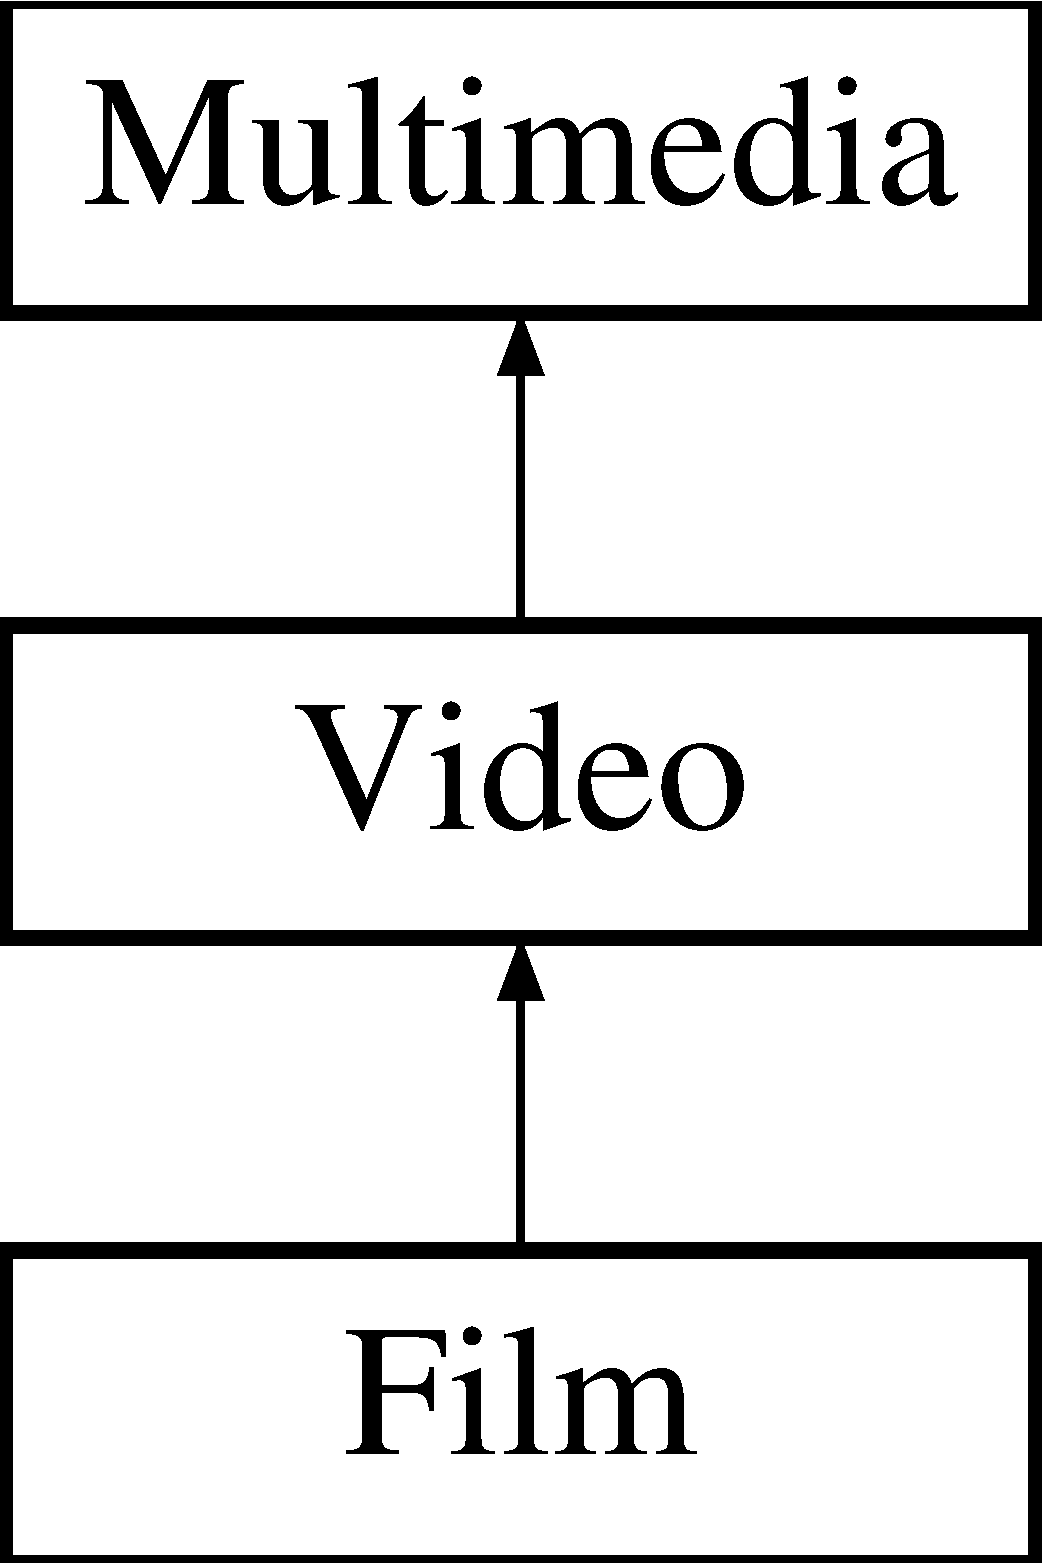
\includegraphics[height=3.000000cm]{class_film}
\end{center}
\end{figure}
\subsection*{Classes}
\begin{DoxyCompactItemize}
\item 
class \hyperlink{class_film_1_1_deleter_film}{Deleter\-Film}
\end{DoxyCompactItemize}
\subsection*{Public Member Functions}
\begin{DoxyCompactItemize}
\item 
virtual unsigned int const $\ast$$\ast$ \hyperlink{class_film_a23040374eae94998b923d861b8c09c7f}{get\-Chapters} (void) const 
\begin{DoxyCompactList}\small\item\em Chapters getter. \end{DoxyCompactList}\item 
virtual void \hyperlink{class_film_a7d9aab418c08d848d27b976c039c3d03}{set\-Chapters} (unsigned int const chapters\mbox{[}$\,$\mbox{]}, unsigned int number\-\_\-chapters)
\begin{DoxyCompactList}\small\item\em Chapters setter. \end{DoxyCompactList}\item 
virtual string \hyperlink{class_film_aac2a77b0b007b5d69c17b26fb0bde949}{print\-Chapters} (void) const 
\begin{DoxyCompactList}\small\item\em Print chapters. \end{DoxyCompactList}\item 
virtual void \hyperlink{class_film_a8b38978dd0bf6ed844627d8e8b63efbe}{write} (ostream \&stream) const 
\begin{DoxyCompactList}\small\item\em Serialize the multimedia object. \end{DoxyCompactList}\item 
virtual void \hyperlink{class_film_a053b2e4cd4b1e1f8dda7cfb1a45d301c}{read} (istream \&stream)
\begin{DoxyCompactList}\small\item\em Read from a serialized object. \end{DoxyCompactList}\end{DoxyCompactItemize}
\subsection*{Protected Member Functions}
\begin{DoxyCompactItemize}
\item 
\hypertarget{class_film_a34c9de2efb9554ce1192e4110d98806b}{{\bfseries Film} (const \hyperlink{class_film}{Film} \&)}\label{class_film_a34c9de2efb9554ce1192e4110d98806b}

\item 
\hyperlink{class_film_aea0f4a8e9741b3c38d4d4d9234ed2ec5}{Film} (void)
\begin{DoxyCompactList}\small\item\em Default Constructor. \end{DoxyCompactList}\item 
\hyperlink{class_film_aa85c4f92943306412e2279c9cd8df7ef}{Film} (string name, unsigned long date, string pathname)
\begin{DoxyCompactList}\small\item\em Constructor with no chapter. \end{DoxyCompactList}\item 
\hyperlink{class_film_abac72e9c84e539851cfe325c6d296acd}{Film} (string name, unsigned long date, string pathname, unsigned int const chapters\mbox{[}$\,$\mbox{]}, unsigned int number\-\_\-chapters)
\begin{DoxyCompactList}\small\item\em Complete constructor. \end{DoxyCompactList}\item 
\hyperlink{class_film_a948efc1e316098a99488235dc99818af}{$\sim$\-Film} (void)
\begin{DoxyCompactList}\small\item\em Destructor. \end{DoxyCompactList}\item 
virtual \hyperlink{class_film}{Film} $\ast$ \hyperlink{class_film_aa0b3eb1efeba4721d86c37ae5e671382}{clone} (void) const 
\begin{DoxyCompactList}\small\item\em Clone the film. \end{DoxyCompactList}\end{DoxyCompactItemize}
\subsection*{Friends}
\begin{DoxyCompactItemize}
\item 
\hypertarget{class_film_a29a97f20d6ded769adf9ecc47158e24f}{class {\bfseries Multimedia\-Manager}}\label{class_film_a29a97f20d6ded769adf9ecc47158e24f}

\item 
\hypertarget{class_film_a400d7bd5ffce270f2e592426ba786a35}{class {\bfseries Deleter\-Film}}\label{class_film_a400d7bd5ffce270f2e592426ba786a35}

\end{DoxyCompactItemize}


\subsection{Detailed Description}
This class represents a film file. 

It inherits from Movie and contains the chapters of the movie. 

\subsection{Constructor \& Destructor Documentation}
\hypertarget{class_film_aea0f4a8e9741b3c38d4d4d9234ed2ec5}{\index{Film@{Film}!Film@{Film}}
\index{Film@{Film}!Film@{Film}}
\subsubsection[{Film}]{\setlength{\rightskip}{0pt plus 5cm}Film\-::\-Film (
\begin{DoxyParamCaption}
\item[{void}]{}
\end{DoxyParamCaption}
)\hspace{0.3cm}{\ttfamily [protected]}}}\label{class_film_aea0f4a8e9741b3c38d4d4d9234ed2ec5}


Default Constructor. 

Creates a default film with no chapter. \hypertarget{class_film_aa85c4f92943306412e2279c9cd8df7ef}{\index{Film@{Film}!Film@{Film}}
\index{Film@{Film}!Film@{Film}}
\subsubsection[{Film}]{\setlength{\rightskip}{0pt plus 5cm}Film\-::\-Film (
\begin{DoxyParamCaption}
\item[{string}]{name, }
\item[{unsigned long}]{date, }
\item[{string}]{pathname}
\end{DoxyParamCaption}
)\hspace{0.3cm}{\ttfamily [protected]}}}\label{class_film_aa85c4f92943306412e2279c9cd8df7ef}


Constructor with no chapter. 

Creates a film with no chapter.


\begin{DoxyParams}{Parameters}
{\em name} & \-: The name of the film. \\
\hline
{\em date} & \-: The date the film was imported. \\
\hline
{\em pathname} & \-: The path to the film. \\
\hline
\end{DoxyParams}
\hypertarget{class_film_abac72e9c84e539851cfe325c6d296acd}{\index{Film@{Film}!Film@{Film}}
\index{Film@{Film}!Film@{Film}}
\subsubsection[{Film}]{\setlength{\rightskip}{0pt plus 5cm}Film\-::\-Film (
\begin{DoxyParamCaption}
\item[{string}]{name, }
\item[{unsigned long}]{date, }
\item[{string}]{pathname, }
\item[{unsigned int const}]{chapters\mbox{[}$\,$\mbox{]}, }
\item[{unsigned int}]{number\-\_\-chapters}
\end{DoxyParamCaption}
)\hspace{0.3cm}{\ttfamily [protected]}}}\label{class_film_abac72e9c84e539851cfe325c6d296acd}


Complete constructor. 

The complete constructor of a film (with chapters).


\begin{DoxyParams}{Parameters}
{\em name} & \-: The name of the film. \\
\hline
{\em date} & \-: The date the film was imported. \\
\hline
{\em pathname} & \-: The path to the film. \\
\hline
{\em chapter} & \-: The vector of the length of each chapter in seconds. \\
\hline
{\em number\-\_\-chapters} & \-: The number of chapter there are. \\
\hline
\end{DoxyParams}
\hypertarget{class_film_a948efc1e316098a99488235dc99818af}{\index{Film@{Film}!$\sim$\-Film@{$\sim$\-Film}}
\index{$\sim$\-Film@{$\sim$\-Film}!Film@{Film}}
\subsubsection[{$\sim$\-Film}]{\setlength{\rightskip}{0pt plus 5cm}Film\-::$\sim$\-Film (
\begin{DoxyParamCaption}
\item[{void}]{}
\end{DoxyParamCaption}
)\hspace{0.3cm}{\ttfamily [protected]}}}\label{class_film_a948efc1e316098a99488235dc99818af}


Destructor. 

Destructor of the class. 

\subsection{Member Function Documentation}
\hypertarget{class_film_aa0b3eb1efeba4721d86c37ae5e671382}{\index{Film@{Film}!clone@{clone}}
\index{clone@{clone}!Film@{Film}}
\subsubsection[{clone}]{\setlength{\rightskip}{0pt plus 5cm}{\bf Film} $\ast$ Film\-::clone (
\begin{DoxyParamCaption}
\item[{void}]{}
\end{DoxyParamCaption}
) const\hspace{0.3cm}{\ttfamily [protected]}, {\ttfamily [virtual]}}}\label{class_film_aa0b3eb1efeba4721d86c37ae5e671382}


Clone the film. 

\begin{DoxyReturn}{Returns}
Return a copy of the given film. 
\end{DoxyReturn}


Reimplemented from \hyperlink{class_video_a450def61b99cd5c338b83cbfa136c25a}{Video}.

\hypertarget{class_film_a23040374eae94998b923d861b8c09c7f}{\index{Film@{Film}!get\-Chapters@{get\-Chapters}}
\index{get\-Chapters@{get\-Chapters}!Film@{Film}}
\subsubsection[{get\-Chapters}]{\setlength{\rightskip}{0pt plus 5cm}unsigned int const $\ast$$\ast$ Film\-::get\-Chapters (
\begin{DoxyParamCaption}
\item[{void}]{}
\end{DoxyParamCaption}
) const\hspace{0.3cm}{\ttfamily [virtual]}}}\label{class_film_a23040374eae94998b923d861b8c09c7f}


Chapters getter. 

Get the tab of the chapters.

\begin{DoxyReturn}{Returns}
A vector with two elements. The first one is a reference to the vector of the chapters and the second one is a reference to the number of chapters. 
\end{DoxyReturn}
\hypertarget{class_film_aac2a77b0b007b5d69c17b26fb0bde949}{\index{Film@{Film}!print\-Chapters@{print\-Chapters}}
\index{print\-Chapters@{print\-Chapters}!Film@{Film}}
\subsubsection[{print\-Chapters}]{\setlength{\rightskip}{0pt plus 5cm}string Film\-::print\-Chapters (
\begin{DoxyParamCaption}
\item[{void}]{}
\end{DoxyParamCaption}
) const\hspace{0.3cm}{\ttfamily [virtual]}}}\label{class_film_aac2a77b0b007b5d69c17b26fb0bde949}


Print chapters. 

Print the chapters of a film. \begin{DoxyReturn}{Returns}
Return a string which contains the chapters list. 
\end{DoxyReturn}
\hypertarget{class_film_a053b2e4cd4b1e1f8dda7cfb1a45d301c}{\index{Film@{Film}!read@{read}}
\index{read@{read}!Film@{Film}}
\subsubsection[{read}]{\setlength{\rightskip}{0pt plus 5cm}void Film\-::read (
\begin{DoxyParamCaption}
\item[{istream \&}]{stream}
\end{DoxyParamCaption}
)\hspace{0.3cm}{\ttfamily [virtual]}}}\label{class_film_a053b2e4cd4b1e1f8dda7cfb1a45d301c}


Read from a serialized object. 


\begin{DoxyParams}{Parameters}
{\em stream} & \-: the input stream where the object will be read. \\
\hline
\end{DoxyParams}


Reimplemented from \hyperlink{class_video_a6be318a4e05ddfdb52fbcc1cab5ab573}{Video}.

\hypertarget{class_film_a7d9aab418c08d848d27b976c039c3d03}{\index{Film@{Film}!set\-Chapters@{set\-Chapters}}
\index{set\-Chapters@{set\-Chapters}!Film@{Film}}
\subsubsection[{set\-Chapters}]{\setlength{\rightskip}{0pt plus 5cm}void Film\-::set\-Chapters (
\begin{DoxyParamCaption}
\item[{unsigned int const}]{chapters\mbox{[}$\,$\mbox{]}, }
\item[{unsigned int}]{number\-\_\-chapters}
\end{DoxyParamCaption}
)\hspace{0.3cm}{\ttfamily [virtual]}}}\label{class_film_a7d9aab418c08d848d27b976c039c3d03}


Chapters setter. 

Set the tab of the chapters.


\begin{DoxyParams}{Parameters}
{\em chapters} & \-: The vector of the length of the chapters. \\
\hline
{\em number\-\_\-chapters} & \-: The number of chapters in the film. \\
\hline
\end{DoxyParams}
\hypertarget{class_film_a8b38978dd0bf6ed844627d8e8b63efbe}{\index{Film@{Film}!write@{write}}
\index{write@{write}!Film@{Film}}
\subsubsection[{write}]{\setlength{\rightskip}{0pt plus 5cm}void Film\-::write (
\begin{DoxyParamCaption}
\item[{ostream \&}]{stream}
\end{DoxyParamCaption}
) const\hspace{0.3cm}{\ttfamily [virtual]}}}\label{class_film_a8b38978dd0bf6ed844627d8e8b63efbe}


Serialize the multimedia object. 


\begin{DoxyParams}{Parameters}
{\em stream} & \-: the output stream where the object will be written. \\
\hline
\end{DoxyParams}


Reimplemented from \hyperlink{class_video_a4bfb8bf83498fa30a6515065559ccbff}{Video}.



The documentation for this class was generated from the following files\-:\begin{DoxyCompactItemize}
\item 
src/headers/film.\-h\item 
src/film.\-cpp\end{DoxyCompactItemize}

\hypertarget{class_group}{\section{Group Class Reference}
\label{class_group}\index{Group@{Group}}
}


This class represents a group of multimedia objects.  




{\ttfamily \#include $<$group.\-h$>$}

Inheritance diagram for Group\-:\begin{figure}[H]
\begin{center}
\leavevmode
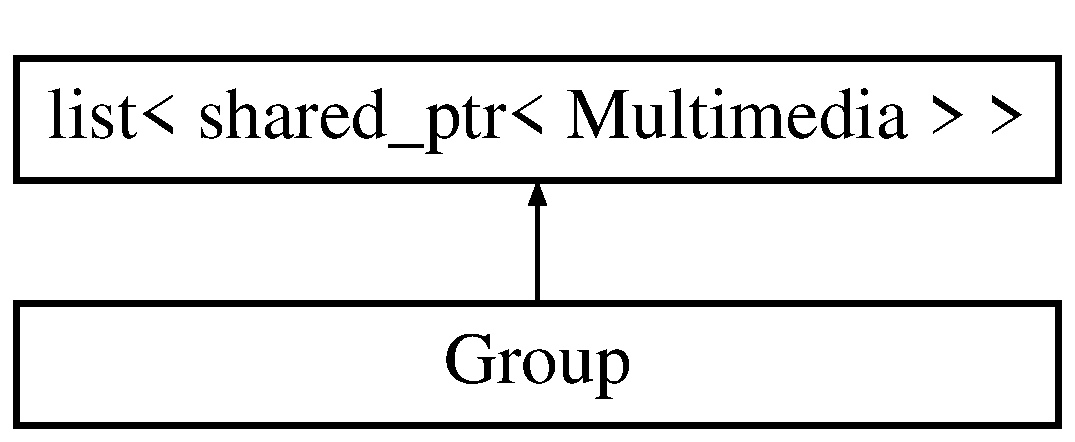
\includegraphics[height=2.000000cm]{class_group}
\end{center}
\end{figure}
\subsection*{Public Member Functions}
\begin{DoxyCompactItemize}
\item 
\hyperlink{class_group_aa6af2d4a3c356458f28074b21da1e4cd}{Group} (void)
\begin{DoxyCompactList}\small\item\em Default Constructor. \end{DoxyCompactList}\item 
\hyperlink{class_group_af214c730661c4bb60beb522c9e727539}{Group} (string name)
\begin{DoxyCompactList}\small\item\em Constructor. \end{DoxyCompactList}\item 
virtual \hyperlink{class_group_a574dd20ac1bc1b887a20674270ef0771}{$\sim$\-Group} (void)
\begin{DoxyCompactList}\small\item\em Default destructor. \end{DoxyCompactList}\item 
virtual string \hyperlink{class_group_a74b6a431e3cc5ea73fe3c827c86124b0}{get\-Name} (void) const 
\begin{DoxyCompactList}\small\item\em Name getter. \end{DoxyCompactList}\item 
virtual void \hyperlink{class_group_abefb2124b85c16a71c4f2507fcc1b929}{set\-Name} (string new\-Name)
\begin{DoxyCompactList}\small\item\em Name setter. \end{DoxyCompactList}\item 
virtual string \hyperlink{class_group_ae6aa5031cd7a0fe6e29d64953dfbb541}{print} (void) const 
\begin{DoxyCompactList}\small\item\em Print all the members. \end{DoxyCompactList}\item 
virtual \hyperlink{class_group}{Group} $\ast$ \hyperlink{class_group_a8a97ac6e71d54db8b11847b584da5e2d}{clone} (void) const 
\begin{DoxyCompactList}\small\item\em Clone the group. \end{DoxyCompactList}\item 
virtual void \hyperlink{class_group_a7906d57eec77398426a976d8c8af7d79}{remove} (string name)
\begin{DoxyCompactList}\small\item\em Remove a multimedia file by name. \end{DoxyCompactList}\item 
virtual void \hyperlink{class_group_abc1a9d8e555c99b902bc7af12c80bd74}{write} (ostream \&stream) const 
\begin{DoxyCompactList}\small\item\em Serializes a group. \end{DoxyCompactList}\item 
virtual void \hyperlink{class_group_a427c00deaef1bd3f04f2986232b68dcd}{read} (istream \&stream, const \hyperlink{class_multimedia_manager}{Multimedia\-Manager} $\ast$manager)
\begin{DoxyCompactList}\small\item\em Deserializes a group. \end{DoxyCompactList}\end{DoxyCompactItemize}


\subsection{Detailed Description}
This class represents a group of multimedia objects. 

The group is represented by a list of multimedia objects, so the methods will be the same. 

\subsection{Constructor \& Destructor Documentation}
\hypertarget{class_group_aa6af2d4a3c356458f28074b21da1e4cd}{\index{Group@{Group}!Group@{Group}}
\index{Group@{Group}!Group@{Group}}
\subsubsection[{Group}]{\setlength{\rightskip}{0pt plus 5cm}Group\-::\-Group (
\begin{DoxyParamCaption}
\item[{void}]{}
\end{DoxyParamCaption}
)}}\label{class_group_aa6af2d4a3c356458f28074b21da1e4cd}


Default Constructor. 

Creates an empty group. \hypertarget{class_group_af214c730661c4bb60beb522c9e727539}{\index{Group@{Group}!Group@{Group}}
\index{Group@{Group}!Group@{Group}}
\subsubsection[{Group}]{\setlength{\rightskip}{0pt plus 5cm}Group\-::\-Group (
\begin{DoxyParamCaption}
\item[{string}]{name}
\end{DoxyParamCaption}
)}}\label{class_group_af214c730661c4bb60beb522c9e727539}


Constructor. 

Creates an empty group.


\begin{DoxyParams}{Parameters}
{\em name} & \-: Name of the group \\
\hline
\end{DoxyParams}
\hypertarget{class_group_a574dd20ac1bc1b887a20674270ef0771}{\index{Group@{Group}!$\sim$\-Group@{$\sim$\-Group}}
\index{$\sim$\-Group@{$\sim$\-Group}!Group@{Group}}
\subsubsection[{$\sim$\-Group}]{\setlength{\rightskip}{0pt plus 5cm}Group\-::$\sim$\-Group (
\begin{DoxyParamCaption}
\item[{void}]{}
\end{DoxyParamCaption}
)\hspace{0.3cm}{\ttfamily [virtual]}}}\label{class_group_a574dd20ac1bc1b887a20674270ef0771}


Default destructor. 

Clean everything before deleting the object. 

\subsection{Member Function Documentation}
\hypertarget{class_group_a8a97ac6e71d54db8b11847b584da5e2d}{\index{Group@{Group}!clone@{clone}}
\index{clone@{clone}!Group@{Group}}
\subsubsection[{clone}]{\setlength{\rightskip}{0pt plus 5cm}{\bf Group} $\ast$ Group\-::clone (
\begin{DoxyParamCaption}
\item[{void}]{}
\end{DoxyParamCaption}
) const\hspace{0.3cm}{\ttfamily [virtual]}}}\label{class_group_a8a97ac6e71d54db8b11847b584da5e2d}


Clone the group. 

\begin{DoxyReturn}{Returns}
A copy of the group. 
\end{DoxyReturn}
\hypertarget{class_group_a74b6a431e3cc5ea73fe3c827c86124b0}{\index{Group@{Group}!get\-Name@{get\-Name}}
\index{get\-Name@{get\-Name}!Group@{Group}}
\subsubsection[{get\-Name}]{\setlength{\rightskip}{0pt plus 5cm}string Group\-::get\-Name (
\begin{DoxyParamCaption}
\item[{void}]{}
\end{DoxyParamCaption}
) const\hspace{0.3cm}{\ttfamily [virtual]}}}\label{class_group_a74b6a431e3cc5ea73fe3c827c86124b0}


Name getter. 

Give the name of the group.

\begin{DoxyReturn}{Returns}
The name of the group. 
\end{DoxyReturn}
\hypertarget{class_group_ae6aa5031cd7a0fe6e29d64953dfbb541}{\index{Group@{Group}!print@{print}}
\index{print@{print}!Group@{Group}}
\subsubsection[{print}]{\setlength{\rightskip}{0pt plus 5cm}string Group\-::print (
\begin{DoxyParamCaption}
\item[{void}]{}
\end{DoxyParamCaption}
) const\hspace{0.3cm}{\ttfamily [virtual]}}}\label{class_group_ae6aa5031cd7a0fe6e29d64953dfbb541}


Print all the members. 

Print the members of the group on the standard output. \hypertarget{class_group_a427c00deaef1bd3f04f2986232b68dcd}{\index{Group@{Group}!read@{read}}
\index{read@{read}!Group@{Group}}
\subsubsection[{read}]{\setlength{\rightskip}{0pt plus 5cm}void Group\-::read (
\begin{DoxyParamCaption}
\item[{istream \&}]{stream, }
\item[{const {\bf Multimedia\-Manager} $\ast$}]{manager}
\end{DoxyParamCaption}
)\hspace{0.3cm}{\ttfamily [virtual]}}}\label{class_group_a427c00deaef1bd3f04f2986232b68dcd}


Deserializes a group. 


\begin{DoxyParams}{Parameters}
{\em stream} & \-: An input stream where the group is read \\
\hline
{\em manager} & \-: The manager where the multimedia files are stored. \\
\hline
\end{DoxyParams}
\hypertarget{class_group_a7906d57eec77398426a976d8c8af7d79}{\index{Group@{Group}!remove@{remove}}
\index{remove@{remove}!Group@{Group}}
\subsubsection[{remove}]{\setlength{\rightskip}{0pt plus 5cm}void Group\-::remove (
\begin{DoxyParamCaption}
\item[{string}]{name}
\end{DoxyParamCaption}
)\hspace{0.3cm}{\ttfamily [virtual]}}}\label{class_group_a7906d57eec77398426a976d8c8af7d79}


Remove a multimedia file by name. 

Remove all the multimedia files in the group with the given name.


\begin{DoxyParams}{Parameters}
{\em name} & \-: the name of the multimedia file to remove. \\
\hline
\end{DoxyParams}
\hypertarget{class_group_abefb2124b85c16a71c4f2507fcc1b929}{\index{Group@{Group}!set\-Name@{set\-Name}}
\index{set\-Name@{set\-Name}!Group@{Group}}
\subsubsection[{set\-Name}]{\setlength{\rightskip}{0pt plus 5cm}void Group\-::set\-Name (
\begin{DoxyParamCaption}
\item[{string}]{new\-Name}
\end{DoxyParamCaption}
)\hspace{0.3cm}{\ttfamily [virtual]}}}\label{class_group_abefb2124b85c16a71c4f2507fcc1b929}


Name setter. 

Set the name of the group.


\begin{DoxyParams}{Parameters}
{\em new\-Name} & \-: the new name of the group. \\
\hline
\end{DoxyParams}
\hypertarget{class_group_abc1a9d8e555c99b902bc7af12c80bd74}{\index{Group@{Group}!write@{write}}
\index{write@{write}!Group@{Group}}
\subsubsection[{write}]{\setlength{\rightskip}{0pt plus 5cm}void Group\-::write (
\begin{DoxyParamCaption}
\item[{ostream \&}]{stream}
\end{DoxyParamCaption}
) const\hspace{0.3cm}{\ttfamily [virtual]}}}\label{class_group_abc1a9d8e555c99b902bc7af12c80bd74}


Serializes a group. 


\begin{DoxyParams}{Parameters}
{\em stream} & \-: An output stream where the group will be written. \\
\hline
\end{DoxyParams}


The documentation for this class was generated from the following files\-:\begin{DoxyCompactItemize}
\item 
src/headers/group.\-h\item 
src/group.\-cpp\end{DoxyCompactItemize}

\hypertarget{classintrusive__ptr}{\section{intrusive\-\_\-ptr$<$ T $>$ Class Template Reference}
\label{classintrusive__ptr}\index{intrusive\-\_\-ptr$<$ T $>$@{intrusive\-\_\-ptr$<$ T $>$}}
}


{\ttfamily \#include $<$intrusive\-\_\-ptr.\-h$>$}

\subsection*{Public Types}
\begin{DoxyCompactItemize}
\item 
\hypertarget{classintrusive__ptr_ae15c9aa35038587012d1b08729cc19c9}{typedef T {\bfseries element\-\_\-type}}\label{classintrusive__ptr_ae15c9aa35038587012d1b08729cc19c9}

\end{DoxyCompactItemize}
\subsection*{Public Member Functions}
\begin{DoxyCompactItemize}
\item 
\hypertarget{classintrusive__ptr_a1a462a7c6f3247828d8360ca04511237}{{\bfseries intrusive\-\_\-ptr} (T $\ast$p, bool add\-\_\-ref=true)}\label{classintrusive__ptr_a1a462a7c6f3247828d8360ca04511237}

\item 
\hypertarget{classintrusive__ptr_a60d33e3607b90c2d7f315d2d0be19735}{{\footnotesize template$<$class U $>$ }\\{\bfseries intrusive\-\_\-ptr} (\hyperlink{classintrusive__ptr}{intrusive\-\_\-ptr}$<$ U $>$ const \&rhs)}\label{classintrusive__ptr_a60d33e3607b90c2d7f315d2d0be19735}

\item 
\hypertarget{classintrusive__ptr_a1a05008b03d6cfb92dfa60515cd848d8}{{\bfseries intrusive\-\_\-ptr} (\hyperlink{classintrusive__ptr}{intrusive\-\_\-ptr} const \&rhs)}\label{classintrusive__ptr_a1a05008b03d6cfb92dfa60515cd848d8}

\item 
\hypertarget{classintrusive__ptr_a3f784a56085dd6e9f711e57a803dd1dc}{{\footnotesize template$<$class U $>$ }\\\hyperlink{classintrusive__ptr}{intrusive\-\_\-ptr} \& {\bfseries operator=} (\hyperlink{classintrusive__ptr}{intrusive\-\_\-ptr}$<$ U $>$ const \&rhs)}\label{classintrusive__ptr_a3f784a56085dd6e9f711e57a803dd1dc}

\item 
\hypertarget{classintrusive__ptr_ae1f058e2b20ea4ef7c3c4c30c8c37694}{\hyperlink{classintrusive__ptr}{intrusive\-\_\-ptr} \& {\bfseries operator=} (\hyperlink{classintrusive__ptr}{intrusive\-\_\-ptr} const \&rhs)}\label{classintrusive__ptr_ae1f058e2b20ea4ef7c3c4c30c8c37694}

\item 
\hypertarget{classintrusive__ptr_acbf9dbecf8e789db853832d84e2c7e19}{\hyperlink{classintrusive__ptr}{intrusive\-\_\-ptr} \& {\bfseries operator=} (T $\ast$rhs)}\label{classintrusive__ptr_acbf9dbecf8e789db853832d84e2c7e19}

\item 
\hypertarget{classintrusive__ptr_ae360b0fffd335b683b350c154922c6db}{void {\bfseries reset} ()}\label{classintrusive__ptr_ae360b0fffd335b683b350c154922c6db}

\item 
\hypertarget{classintrusive__ptr_a81e2fb688afba02de9ecf2006caeb62e}{void {\bfseries reset} (T $\ast$rhs)}\label{classintrusive__ptr_a81e2fb688afba02de9ecf2006caeb62e}

\item 
\hypertarget{classintrusive__ptr_a70192c07e3ff5035942095a5d2d97c34}{T $\ast$ {\bfseries get} () const }\label{classintrusive__ptr_a70192c07e3ff5035942095a5d2d97c34}

\item 
\hypertarget{classintrusive__ptr_a63f7f0b02c547127f9f68ecdb01f7aa6}{T \& {\bfseries operator$\ast$} () const }\label{classintrusive__ptr_a63f7f0b02c547127f9f68ecdb01f7aa6}

\item 
\hypertarget{classintrusive__ptr_a4756c9e89a1a057e2c911d8224197d31}{T $\ast$ {\bfseries operator-\/$>$} () const }\label{classintrusive__ptr_a4756c9e89a1a057e2c911d8224197d31}

\item 
\hypertarget{classintrusive__ptr_a1a71711829594617e226fada9b7ef351}{{\bfseries operator unspecified\-\_\-bool\-\_\-type} () const }\label{classintrusive__ptr_a1a71711829594617e226fada9b7ef351}

\item 
\hypertarget{classintrusive__ptr_aee167762c6829dac96f664b4ab505e39}{bool {\bfseries operator!} () const }\label{classintrusive__ptr_aee167762c6829dac96f664b4ab505e39}

\item 
\hypertarget{classintrusive__ptr_a95826a79f706bc5c6b9fd28ae334e974}{void {\bfseries swap} (\hyperlink{classintrusive__ptr}{intrusive\-\_\-ptr} \&rhs)}\label{classintrusive__ptr_a95826a79f706bc5c6b9fd28ae334e974}

\end{DoxyCompactItemize}


\subsection{Detailed Description}
\subsubsection*{template$<$class T$>$class intrusive\-\_\-ptr$<$ T $>$}

\hyperlink{classintrusive__ptr}{intrusive\-\_\-ptr}\-: a smart pointer that uses intrusive reference counting. Relies on unqualified calls to 
\begin{DoxyPre}
     void intrusive\_ptr\_add\_ref(T * p);
     void intrusive\_ptr\_release(T * p);
\end{DoxyPre}
 (p != 0)

The object is responsible for destroying itself. 

The documentation for this class was generated from the following file\-:\begin{DoxyCompactItemize}
\item 
src/headers/intrusive\-\_\-ptr.\-h\end{DoxyCompactItemize}

\hypertarget{class_main_window}{\section{Main\-Window Class Reference}
\label{class_main_window}\index{Main\-Window@{Main\-Window}}
}


This is the main window of the program.  


Inheritance diagram for Main\-Window\-:\begin{figure}[H]
\begin{center}
\leavevmode
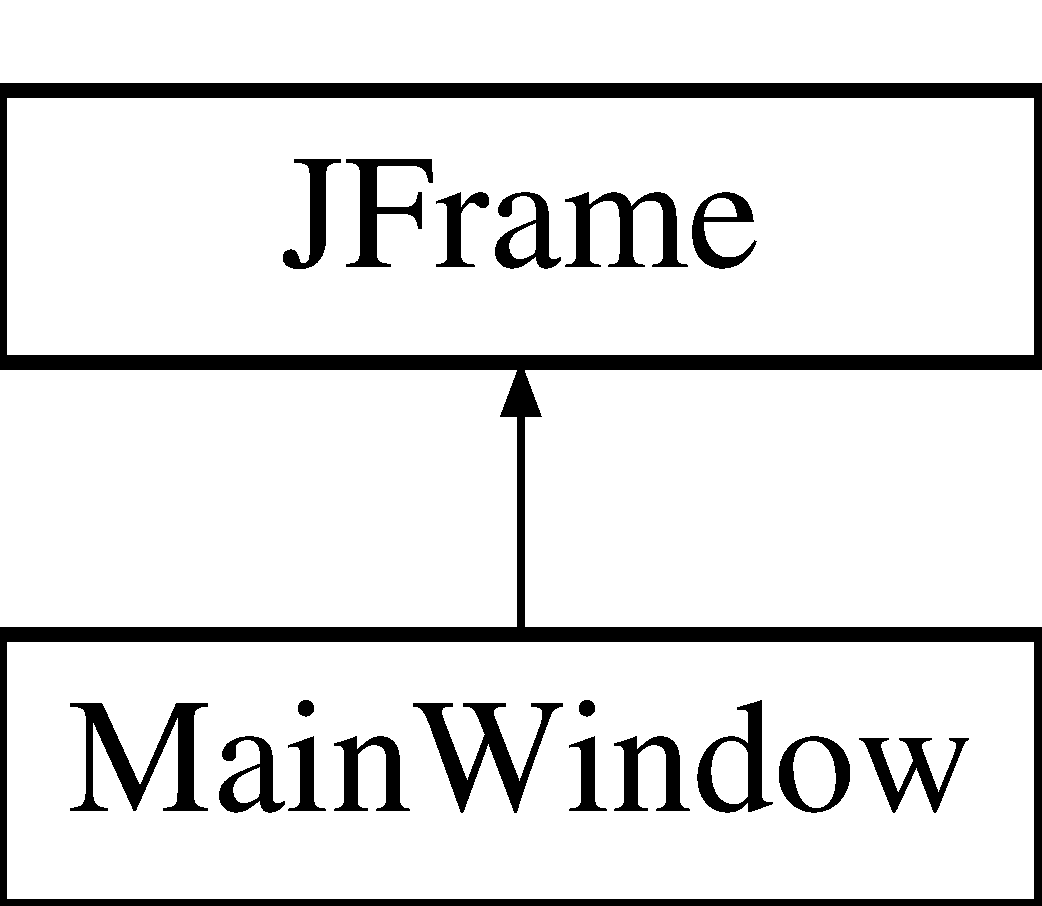
\includegraphics[height=2.000000cm]{class_main_window}
\end{center}
\end{figure}
\subsection*{Public Member Functions}
\begin{DoxyCompactItemize}
\item 
\hyperlink{class_main_window_aa4faae6551f241dfe3ccc9061a33eb5a}{Main\-Window} (\hyperlink{class_client}{Client} cl)
\begin{DoxyCompactList}\small\item\em Constructor. \end{DoxyCompactList}\end{DoxyCompactItemize}


\subsection{Detailed Description}
This is the main window of the program. 

\subsection{Constructor \& Destructor Documentation}
\hypertarget{class_main_window_aa4faae6551f241dfe3ccc9061a33eb5a}{\index{Main\-Window@{Main\-Window}!Main\-Window@{Main\-Window}}
\index{Main\-Window@{Main\-Window}!MainWindow@{Main\-Window}}
\subsubsection[{Main\-Window}]{\setlength{\rightskip}{0pt plus 5cm}Main\-Window.\-Main\-Window (
\begin{DoxyParamCaption}
\item[{{\bf Client}}]{cl}
\end{DoxyParamCaption}
)\hspace{0.3cm}{\ttfamily [inline]}}}\label{class_main_window_aa4faae6551f241dfe3ccc9061a33eb5a}


Constructor. 

Creates the main window. 

The documentation for this class was generated from the following file\-:\begin{DoxyCompactItemize}
\item 
src/graphique/Main\-Window.\-java\end{DoxyCompactItemize}

\hypertarget{class_multimedia}{\section{Multimedia Class Reference}
\label{class_multimedia}\index{Multimedia@{Multimedia}}
}


This class represents a multimedia file.  




{\ttfamily \#include $<$multimedia.\-h$>$}

\subsection*{Public Member Functions}
\begin{DoxyCompactItemize}
\item 
\hyperlink{class_multimedia_af613763f6779c2e75fce0749b9a8a734}{Multimedia} (void)
\begin{DoxyCompactList}\small\item\em Default Constructor. \end{DoxyCompactList}\item 
\hyperlink{class_multimedia_a4b955c8674fb9ff39e57fd178f08bada}{Multimedia} (string name, unsigned long date, string pathname)
\begin{DoxyCompactList}\small\item\em Constructor. \end{DoxyCompactList}\item 
\hyperlink{class_multimedia_a53798cec796a3aa8df3a35dfaa37bfe7}{$\sim$\-Multimedia} (void)
\begin{DoxyCompactList}\small\item\em Destructor. \end{DoxyCompactList}\item 
virtual string \hyperlink{class_multimedia_a8cc74dd745e553a881e6d5b210a542f6}{get\-Name} (void) const 
\begin{DoxyCompactList}\small\item\em Name getter. \end{DoxyCompactList}\item 
virtual unsigned long \hyperlink{class_multimedia_a8c5b6295faee6c9690a513dd0f4b4a79}{get\-Date} (void) const 
\begin{DoxyCompactList}\small\item\em Date getter. \end{DoxyCompactList}\item 
virtual string \hyperlink{class_multimedia_a6cff0cb9e8a32d2589c77ebf37250da3}{get\-Pathname} (void) const 
\begin{DoxyCompactList}\small\item\em Pathname getter. \end{DoxyCompactList}\item 
virtual void \hyperlink{class_multimedia_a7af3fbc7c6f5eab1a70608066f05d03d}{set\-Name} (string new\-Name)
\begin{DoxyCompactList}\small\item\em Name setter. \end{DoxyCompactList}\item 
virtual void \hyperlink{class_multimedia_a14abd8762b4d64cba41822f2b8ad434f}{set\-Date} (unsigned long new\-Date)
\begin{DoxyCompactList}\small\item\em Date setter. \end{DoxyCompactList}\item 
virtual void \hyperlink{class_multimedia_a3e06f151e9fce4cad4f74e4b92276929}{set\-Pathname} (string new\-Pathname)
\begin{DoxyCompactList}\small\item\em Path setter. \end{DoxyCompactList}\item 
virtual void \hyperlink{class_multimedia_a1b1b48641e51f3d840cf68634554c85a}{print} (void) const 
\begin{DoxyCompactList}\small\item\em Print description. \end{DoxyCompactList}\end{DoxyCompactItemize}


\subsection{Detailed Description}
This class represents a multimedia file. 

All multimedia files inherit from this class. 

\subsection{Constructor \& Destructor Documentation}
\hypertarget{class_multimedia_af613763f6779c2e75fce0749b9a8a734}{\index{Multimedia@{Multimedia}!Multimedia@{Multimedia}}
\index{Multimedia@{Multimedia}!Multimedia@{Multimedia}}
\subsubsection[{Multimedia}]{\setlength{\rightskip}{0pt plus 5cm}Multimedia\-::\-Multimedia (
\begin{DoxyParamCaption}
\item[{void}]{}
\end{DoxyParamCaption}
)}}\label{class_multimedia_af613763f6779c2e75fce0749b9a8a734}


Default Constructor. 

Creates a default multimedia object. \hypertarget{class_multimedia_a4b955c8674fb9ff39e57fd178f08bada}{\index{Multimedia@{Multimedia}!Multimedia@{Multimedia}}
\index{Multimedia@{Multimedia}!Multimedia@{Multimedia}}
\subsubsection[{Multimedia}]{\setlength{\rightskip}{0pt plus 5cm}Multimedia\-::\-Multimedia (
\begin{DoxyParamCaption}
\item[{string}]{name, }
\item[{unsigned long}]{date, }
\item[{string}]{pathname}
\end{DoxyParamCaption}
)}}\label{class_multimedia_a4b955c8674fb9ff39e57fd178f08bada}


Constructor. 

Constructor of the \hyperlink{class_multimedia}{Multimedia} class.


\begin{DoxyParams}{Parameters}
{\em name} & \-: Name of the multimedia file \\
\hline
{\em date} & \-: Date when the file is added in seconds \\
\hline
{\em pathname} & \-: Path to the file \\
\hline
\end{DoxyParams}
\hypertarget{class_multimedia_a53798cec796a3aa8df3a35dfaa37bfe7}{\index{Multimedia@{Multimedia}!$\sim$\-Multimedia@{$\sim$\-Multimedia}}
\index{$\sim$\-Multimedia@{$\sim$\-Multimedia}!Multimedia@{Multimedia}}
\subsubsection[{$\sim$\-Multimedia}]{\setlength{\rightskip}{0pt plus 5cm}Multimedia\-::$\sim$\-Multimedia (
\begin{DoxyParamCaption}
\item[{void}]{}
\end{DoxyParamCaption}
)}}\label{class_multimedia_a53798cec796a3aa8df3a35dfaa37bfe7}


Destructor. 

Default destructor of this class. 

\subsection{Member Function Documentation}
\hypertarget{class_multimedia_a8c5b6295faee6c9690a513dd0f4b4a79}{\index{Multimedia@{Multimedia}!get\-Date@{get\-Date}}
\index{get\-Date@{get\-Date}!Multimedia@{Multimedia}}
\subsubsection[{get\-Date}]{\setlength{\rightskip}{0pt plus 5cm}unsigned long Multimedia\-::get\-Date (
\begin{DoxyParamCaption}
\item[{void}]{}
\end{DoxyParamCaption}
) const\hspace{0.3cm}{\ttfamily [virtual]}}}\label{class_multimedia_a8c5b6295faee6c9690a513dd0f4b4a79}


Date getter. 

Get the date the file was added.

\begin{DoxyReturn}{Returns}
The date the file was imported in seconds. 
\end{DoxyReturn}
\hypertarget{class_multimedia_a8cc74dd745e553a881e6d5b210a542f6}{\index{Multimedia@{Multimedia}!get\-Name@{get\-Name}}
\index{get\-Name@{get\-Name}!Multimedia@{Multimedia}}
\subsubsection[{get\-Name}]{\setlength{\rightskip}{0pt plus 5cm}string Multimedia\-::get\-Name (
\begin{DoxyParamCaption}
\item[{void}]{}
\end{DoxyParamCaption}
) const\hspace{0.3cm}{\ttfamily [virtual]}}}\label{class_multimedia_a8cc74dd745e553a881e6d5b210a542f6}


Name getter. 

Get the name of the file.

\begin{DoxyReturn}{Returns}
The name of file 
\end{DoxyReturn}
\hypertarget{class_multimedia_a6cff0cb9e8a32d2589c77ebf37250da3}{\index{Multimedia@{Multimedia}!get\-Pathname@{get\-Pathname}}
\index{get\-Pathname@{get\-Pathname}!Multimedia@{Multimedia}}
\subsubsection[{get\-Pathname}]{\setlength{\rightskip}{0pt plus 5cm}string Multimedia\-::get\-Pathname (
\begin{DoxyParamCaption}
\item[{void}]{}
\end{DoxyParamCaption}
) const\hspace{0.3cm}{\ttfamily [virtual]}}}\label{class_multimedia_a6cff0cb9e8a32d2589c77ebf37250da3}


Pathname getter. 

Get the path to the file.

\begin{DoxyReturn}{Returns}
The path to the file 
\end{DoxyReturn}
\hypertarget{class_multimedia_a1b1b48641e51f3d840cf68634554c85a}{\index{Multimedia@{Multimedia}!print@{print}}
\index{print@{print}!Multimedia@{Multimedia}}
\subsubsection[{print}]{\setlength{\rightskip}{0pt plus 5cm}void Multimedia\-::print (
\begin{DoxyParamCaption}
\item[{void}]{}
\end{DoxyParamCaption}
) const\hspace{0.3cm}{\ttfamily [virtual]}}}\label{class_multimedia_a1b1b48641e51f3d840cf68634554c85a}


Print description. 

Print the description of the file to the standard output \hypertarget{class_multimedia_a14abd8762b4d64cba41822f2b8ad434f}{\index{Multimedia@{Multimedia}!set\-Date@{set\-Date}}
\index{set\-Date@{set\-Date}!Multimedia@{Multimedia}}
\subsubsection[{set\-Date}]{\setlength{\rightskip}{0pt plus 5cm}void Multimedia\-::set\-Date (
\begin{DoxyParamCaption}
\item[{unsigned long}]{new\-Date}
\end{DoxyParamCaption}
)\hspace{0.3cm}{\ttfamily [virtual]}}}\label{class_multimedia_a14abd8762b4d64cba41822f2b8ad434f}


Date setter. 

Set the date associated to the file.


\begin{DoxyParams}{Parameters}
{\em new\-Date} & \-: the new value of the date in seconds. \\
\hline
\end{DoxyParams}
\hypertarget{class_multimedia_a7af3fbc7c6f5eab1a70608066f05d03d}{\index{Multimedia@{Multimedia}!set\-Name@{set\-Name}}
\index{set\-Name@{set\-Name}!Multimedia@{Multimedia}}
\subsubsection[{set\-Name}]{\setlength{\rightskip}{0pt plus 5cm}void Multimedia\-::set\-Name (
\begin{DoxyParamCaption}
\item[{string}]{new\-Name}
\end{DoxyParamCaption}
)\hspace{0.3cm}{\ttfamily [virtual]}}}\label{class_multimedia_a7af3fbc7c6f5eab1a70608066f05d03d}


Name setter. 

Set the name of the file.


\begin{DoxyParams}{Parameters}
{\em new\-Name} & \-: the new name of the file \\
\hline
\end{DoxyParams}
\hypertarget{class_multimedia_a3e06f151e9fce4cad4f74e4b92276929}{\index{Multimedia@{Multimedia}!set\-Pathname@{set\-Pathname}}
\index{set\-Pathname@{set\-Pathname}!Multimedia@{Multimedia}}
\subsubsection[{set\-Pathname}]{\setlength{\rightskip}{0pt plus 5cm}void Multimedia\-::set\-Pathname (
\begin{DoxyParamCaption}
\item[{string}]{new\-Pathname}
\end{DoxyParamCaption}
)\hspace{0.3cm}{\ttfamily [virtual]}}}\label{class_multimedia_a3e06f151e9fce4cad4f74e4b92276929}


Path setter. 


\begin{DoxyParams}{Parameters}
{\em new\-Pathname} & \-: the new path to the file. \\
\hline
\end{DoxyParams}


The documentation for this class was generated from the following files\-:\begin{DoxyCompactItemize}
\item 
src/headers/multimedia.\-h\item 
src/multimedia.\-cpp\end{DoxyCompactItemize}

\hypertarget{class_multimedia_manager}{\section{Multimedia\-Manager Class Reference}
\label{class_multimedia_manager}\index{Multimedia\-Manager@{Multimedia\-Manager}}
}


Manages the multimedia files and groups.  




{\ttfamily \#include $<$multimedia\-\_\-manager.\-h$>$}

\subsection*{Public Member Functions}
\begin{DoxyCompactItemize}
\item 
virtual \hyperlink{class_multimedia_manager_acffc32fc3ac866e8aa01408c4dd8fce3}{$\sim$\-Multimedia\-Manager} (void)
\begin{DoxyCompactList}\small\item\em Destructor. \end{DoxyCompactList}\item 
virtual shared\-\_\-ptr$<$ \hyperlink{class_photo}{Photo} $>$ \hyperlink{class_multimedia_manager_a835209002b726811b325ef326b3fa6fd}{create\-\_\-photo} (void)
\begin{DoxyCompactList}\small\item\em Creates a default photo. \end{DoxyCompactList}\item 
virtual shared\-\_\-ptr$<$ \hyperlink{class_photo}{Photo} $>$ \hyperlink{class_multimedia_manager_a26f3f416ddd521a4be3998cd8a766c09}{create\-\_\-photo} (const string \&name, unsigned long date, const string \&pathname, const string \&place)
\begin{DoxyCompactList}\small\item\em Creates a photo file. \end{DoxyCompactList}\item 
virtual shared\-\_\-ptr$<$ \hyperlink{class_photo}{Photo} $>$ \hyperlink{class_multimedia_manager_a6db30d90657a2e9d3aa00a316338ccff}{create\-\_\-photo} (istream \&is)
\begin{DoxyCompactList}\small\item\em Deserialize a photo. \end{DoxyCompactList}\item 
virtual shared\-\_\-ptr$<$ \hyperlink{class_video}{Video} $>$ \hyperlink{class_multimedia_manager_ae18114802de3529b7d0d20772a7288da}{create\-\_\-video} (void)
\begin{DoxyCompactList}\small\item\em Creates a default video. \end{DoxyCompactList}\item 
virtual shared\-\_\-ptr$<$ \hyperlink{class_video}{Video} $>$ \hyperlink{class_multimedia_manager_a3d5cbae8789ee6576da1b92a6a136725}{create\-\_\-video} (const string \&name, unsigned long date, const string \&pathname, unsigned int length)
\begin{DoxyCompactList}\small\item\em Creates a video. \end{DoxyCompactList}\item 
virtual shared\-\_\-ptr$<$ \hyperlink{class_video}{Video} $>$ \hyperlink{class_multimedia_manager_ab0737cc478f5060c9da0a33762f2f34c}{create\-\_\-video} (istream \&is)
\begin{DoxyCompactList}\small\item\em Deserialize a video. \end{DoxyCompactList}\item 
virtual shared\-\_\-ptr$<$ \hyperlink{class_film}{Film} $>$ \hyperlink{class_multimedia_manager_af33b0c0a9adde3856d783d7ca99d9267}{create\-\_\-film} (void)
\begin{DoxyCompactList}\small\item\em Creates a default film. \end{DoxyCompactList}\item 
virtual shared\-\_\-ptr$<$ \hyperlink{class_film}{Film} $>$ \hyperlink{class_multimedia_manager_a433256dd37e58487f960558bcd8cb8fc}{create\-\_\-film} (const string \&name, unsigned long date, const string \&pathname)
\begin{DoxyCompactList}\small\item\em Creates a film with no chapter. \end{DoxyCompactList}\item 
virtual shared\-\_\-ptr$<$ \hyperlink{class_film}{Film} $>$ \hyperlink{class_multimedia_manager_a6437bb9bed0f47caa5f838ae7d9e972c}{create\-\_\-film} (const string \&name, unsigned long date, const string \&pathname, unsigned int const chapters\mbox{[}$\,$\mbox{]}, unsigned int number\-\_\-chapters)
\begin{DoxyCompactList}\small\item\em Creates a film. \end{DoxyCompactList}\item 
virtual shared\-\_\-ptr$<$ \hyperlink{class_film}{Film} $>$ \hyperlink{class_multimedia_manager_afff770e7acd58cf182ed1ec0901ed69b}{create\-\_\-film} (istream \&is)
\begin{DoxyCompactList}\small\item\em Deserialize a film. \end{DoxyCompactList}\item 
virtual shared\-\_\-ptr$<$ \hyperlink{class_group}{Group} $>$ \hyperlink{class_multimedia_manager_af19f5851053008905770ec23168891c4}{create} (const \hyperlink{class_group}{Group} \&group)
\begin{DoxyCompactList}\small\item\em Creates a group. \end{DoxyCompactList}\item 
virtual shared\-\_\-ptr$<$ \hyperlink{class_group}{Group} $>$ \hyperlink{class_multimedia_manager_a5ebb82c40be17ec58797aaee94fb6238}{create\-\_\-group} ()
\begin{DoxyCompactList}\small\item\em Creates a default group. \end{DoxyCompactList}\item 
virtual shared\-\_\-ptr$<$ \hyperlink{class_group}{Group} $>$ \hyperlink{class_multimedia_manager_a0f9efa126e6f1e43b5256fe54db5f5d1}{create\-\_\-group} (const string \&)
\begin{DoxyCompactList}\small\item\em Creates a group. \end{DoxyCompactList}\item 
virtual shared\-\_\-ptr$<$ \hyperlink{class_group}{Group} $>$ \hyperlink{class_multimedia_manager_ad3b4a69b6dcf13fad2aa016c68fcf357}{create\-\_\-group} (istream \&is)
\begin{DoxyCompactList}\small\item\em Creates a group from a stream. \end{DoxyCompactList}\item 
virtual void \hyperlink{class_multimedia_manager_aaeb480df4f0ef43fe08e820e44006eb9}{remove\-\_\-multimedia} (const string \&name)
\begin{DoxyCompactList}\small\item\em Remove a multimedia file. \end{DoxyCompactList}\item 
virtual void \hyperlink{class_multimedia_manager_a8a6ebd815c8b19b357f2440f943a6dcb}{remove\-\_\-group} (const string \&name)
\begin{DoxyCompactList}\small\item\em Remove a group. \end{DoxyCompactList}\item 
virtual string \hyperlink{class_multimedia_manager_aa936143b04d97ea3b74c7016482512b9}{search\-\_\-multimedia} (const string \&name) const 
\begin{DoxyCompactList}\small\item\em Search a multimedia file and print it. \end{DoxyCompactList}\item 
virtual shared\-\_\-ptr$<$ \hyperlink{class_multimedia}{Multimedia} $>$ \hyperlink{class_multimedia_manager_a6e6fb41d321267cde7229fe7d1fa3ba7}{search\-\_\-multimedia\-\_\-ptr} (const string \&name) const 
\begin{DoxyCompactList}\small\item\em Search a multimedia file and print its pointer. \end{DoxyCompactList}\item 
virtual string \hyperlink{class_multimedia_manager_a39a4fc5cd5163e01f112bd474ef76e1b}{search\-\_\-group} (const string \&name) const 
\begin{DoxyCompactList}\small\item\em Search a group and print it. \end{DoxyCompactList}\item 
virtual void \hyperlink{class_multimedia_manager_ad99e3dfbf0ad3f9e1a7423f89ad0f45a}{play} (const string \&name) const 
\begin{DoxyCompactList}\small\item\em Play a multimedia file. \end{DoxyCompactList}\item 
virtual void \hyperlink{class_multimedia_manager_a11c103cd8ec48581c81a522629d536b7}{write} (const string \&name) const 
\begin{DoxyCompactList}\small\item\em Serialize the manager with its content. \end{DoxyCompactList}\item 
virtual void \hyperlink{class_multimedia_manager_ae6830452883cc26ab9f89d20c024553a}{read} (const string \&name)
\begin{DoxyCompactList}\small\item\em Read a manager. \end{DoxyCompactList}\end{DoxyCompactItemize}


\subsection{Detailed Description}
Manages the multimedia files and groups. 

This is the main interface to create \& delete multimedia files. It also allows to create, delete a group. 

\subsection{Constructor \& Destructor Documentation}
\hypertarget{class_multimedia_manager_acffc32fc3ac866e8aa01408c4dd8fce3}{\index{Multimedia\-Manager@{Multimedia\-Manager}!$\sim$\-Multimedia\-Manager@{$\sim$\-Multimedia\-Manager}}
\index{$\sim$\-Multimedia\-Manager@{$\sim$\-Multimedia\-Manager}!MultimediaManager@{Multimedia\-Manager}}
\subsubsection[{$\sim$\-Multimedia\-Manager}]{\setlength{\rightskip}{0pt plus 5cm}Multimedia\-Manager\-::$\sim$\-Multimedia\-Manager (
\begin{DoxyParamCaption}
\item[{void}]{}
\end{DoxyParamCaption}
)\hspace{0.3cm}{\ttfamily [virtual]}}}\label{class_multimedia_manager_acffc32fc3ac866e8aa01408c4dd8fce3}


Destructor. 

Called before destruction. 

\subsection{Member Function Documentation}
\hypertarget{class_multimedia_manager_af19f5851053008905770ec23168891c4}{\index{Multimedia\-Manager@{Multimedia\-Manager}!create@{create}}
\index{create@{create}!MultimediaManager@{Multimedia\-Manager}}
\subsubsection[{create}]{\setlength{\rightskip}{0pt plus 5cm}shared\-\_\-ptr$<$ {\bf Group} $>$ Multimedia\-Manager\-::create (
\begin{DoxyParamCaption}
\item[{const {\bf Group} \&}]{group}
\end{DoxyParamCaption}
)\hspace{0.3cm}{\ttfamily [virtual]}}}\label{class_multimedia_manager_af19f5851053008905770ec23168891c4}


Creates a group. 

Create a new group and add it to the manager.

 
\begin{DoxyParams}{Parameters}
{\em group} & \-: the group to create.\\
\hline
\end{DoxyParams}
\begin{DoxyReturn}{Returns}
A shared pointer to the group created. 
\end{DoxyReturn}
\hypertarget{class_multimedia_manager_af33b0c0a9adde3856d783d7ca99d9267}{\index{Multimedia\-Manager@{Multimedia\-Manager}!create\-\_\-film@{create\-\_\-film}}
\index{create\-\_\-film@{create\-\_\-film}!MultimediaManager@{Multimedia\-Manager}}
\subsubsection[{create\-\_\-film}]{\setlength{\rightskip}{0pt plus 5cm}shared\-\_\-ptr$<$ {\bf Film} $>$ Multimedia\-Manager\-::create\-\_\-film (
\begin{DoxyParamCaption}
\item[{void}]{}
\end{DoxyParamCaption}
)\hspace{0.3cm}{\ttfamily [virtual]}}}\label{class_multimedia_manager_af33b0c0a9adde3856d783d7ca99d9267}


Creates a default film. 

Add a film file in the manager.

\begin{DoxyReturn}{Returns}
A shared pointer to the object created. 
\end{DoxyReturn}
\hypertarget{class_multimedia_manager_a433256dd37e58487f960558bcd8cb8fc}{\index{Multimedia\-Manager@{Multimedia\-Manager}!create\-\_\-film@{create\-\_\-film}}
\index{create\-\_\-film@{create\-\_\-film}!MultimediaManager@{Multimedia\-Manager}}
\subsubsection[{create\-\_\-film}]{\setlength{\rightskip}{0pt plus 5cm}shared\-\_\-ptr$<$ {\bf Film} $>$ Multimedia\-Manager\-::create\-\_\-film (
\begin{DoxyParamCaption}
\item[{const string \&}]{name, }
\item[{unsigned long}]{date, }
\item[{const string \&}]{pathname}
\end{DoxyParamCaption}
)\hspace{0.3cm}{\ttfamily [virtual]}}}\label{class_multimedia_manager_a433256dd37e58487f960558bcd8cb8fc}


Creates a film with no chapter. 

Add a film file in the manager.


\begin{DoxyParams}{Parameters}
{\em name} & \-: Name of the film. \\
\hline
{\em date} & \-: The date when the file was created. \\
\hline
{\em pathname} & \-: The path to the file.\\
\hline
\end{DoxyParams}
\begin{DoxyReturn}{Returns}
A shared pointer to the object created. 
\end{DoxyReturn}
\hypertarget{class_multimedia_manager_a6437bb9bed0f47caa5f838ae7d9e972c}{\index{Multimedia\-Manager@{Multimedia\-Manager}!create\-\_\-film@{create\-\_\-film}}
\index{create\-\_\-film@{create\-\_\-film}!MultimediaManager@{Multimedia\-Manager}}
\subsubsection[{create\-\_\-film}]{\setlength{\rightskip}{0pt plus 5cm}shared\-\_\-ptr$<$ {\bf Film} $>$ Multimedia\-Manager\-::create\-\_\-film (
\begin{DoxyParamCaption}
\item[{const string \&}]{name, }
\item[{unsigned long}]{date, }
\item[{const string \&}]{pathname, }
\item[{unsigned int const}]{chapters\mbox{[}$\,$\mbox{]}, }
\item[{unsigned int}]{number\-\_\-chapters}
\end{DoxyParamCaption}
)\hspace{0.3cm}{\ttfamily [virtual]}}}\label{class_multimedia_manager_a6437bb9bed0f47caa5f838ae7d9e972c}


Creates a film. 

Add a film file in the manager.


\begin{DoxyParams}{Parameters}
{\em name} & \-: Name of the film. \\
\hline
{\em date} & \-: The date when the file was created. \\
\hline
{\em pathname} & \-: The path to the file. \\
\hline
{\em chapters} & \-: The array the the length of the chapters. \\
\hline
{\em number\-\_\-chapters} & \-: The number of chapter in the film.\\
\hline
\end{DoxyParams}
\begin{DoxyReturn}{Returns}
A shared pointer to the object created. 
\end{DoxyReturn}
\hypertarget{class_multimedia_manager_afff770e7acd58cf182ed1ec0901ed69b}{\index{Multimedia\-Manager@{Multimedia\-Manager}!create\-\_\-film@{create\-\_\-film}}
\index{create\-\_\-film@{create\-\_\-film}!MultimediaManager@{Multimedia\-Manager}}
\subsubsection[{create\-\_\-film}]{\setlength{\rightskip}{0pt plus 5cm}shared\-\_\-ptr$<$ {\bf Film} $>$ Multimedia\-Manager\-::create\-\_\-film (
\begin{DoxyParamCaption}
\item[{istream \&}]{is}
\end{DoxyParamCaption}
)\hspace{0.3cm}{\ttfamily [virtual]}}}\label{class_multimedia_manager_afff770e7acd58cf182ed1ec0901ed69b}


Deserialize a film. 


\begin{DoxyParams}{Parameters}
{\em The} & stream where the film will be read. \\
\hline
\end{DoxyParams}
\begin{DoxyReturn}{Returns}
A shared pointer to the object created. 
\end{DoxyReturn}
\hypertarget{class_multimedia_manager_a5ebb82c40be17ec58797aaee94fb6238}{\index{Multimedia\-Manager@{Multimedia\-Manager}!create\-\_\-group@{create\-\_\-group}}
\index{create\-\_\-group@{create\-\_\-group}!MultimediaManager@{Multimedia\-Manager}}
\subsubsection[{create\-\_\-group}]{\setlength{\rightskip}{0pt plus 5cm}shared\-\_\-ptr$<$ {\bf Group} $>$ Multimedia\-Manager\-::create\-\_\-group (
\begin{DoxyParamCaption}
{}
\end{DoxyParamCaption}
)\hspace{0.3cm}{\ttfamily [virtual]}}}\label{class_multimedia_manager_a5ebb82c40be17ec58797aaee94fb6238}


Creates a default group. 

Create a new group and add it to the manager.

\begin{DoxyReturn}{Returns}
A shared pointer to the group created. 
\end{DoxyReturn}
\hypertarget{class_multimedia_manager_a0f9efa126e6f1e43b5256fe54db5f5d1}{\index{Multimedia\-Manager@{Multimedia\-Manager}!create\-\_\-group@{create\-\_\-group}}
\index{create\-\_\-group@{create\-\_\-group}!MultimediaManager@{Multimedia\-Manager}}
\subsubsection[{create\-\_\-group}]{\setlength{\rightskip}{0pt plus 5cm}shared\-\_\-ptr$<$ {\bf Group} $>$ Multimedia\-Manager\-::create\-\_\-group (
\begin{DoxyParamCaption}
\item[{const string \&}]{name}
\end{DoxyParamCaption}
)\hspace{0.3cm}{\ttfamily [virtual]}}}\label{class_multimedia_manager_a0f9efa126e6f1e43b5256fe54db5f5d1}


Creates a group. 

Create a new group and add it to the manager.

 
\begin{DoxyParams}{Parameters}
{\em group} & \-: the name of the group to create.\\
\hline
\end{DoxyParams}
\begin{DoxyReturn}{Returns}
A shared pointer to the group created. 
\end{DoxyReturn}
\hypertarget{class_multimedia_manager_ad3b4a69b6dcf13fad2aa016c68fcf357}{\index{Multimedia\-Manager@{Multimedia\-Manager}!create\-\_\-group@{create\-\_\-group}}
\index{create\-\_\-group@{create\-\_\-group}!MultimediaManager@{Multimedia\-Manager}}
\subsubsection[{create\-\_\-group}]{\setlength{\rightskip}{0pt plus 5cm}shared\-\_\-ptr$<$ {\bf Group} $>$ Multimedia\-Manager\-::create\-\_\-group (
\begin{DoxyParamCaption}
\item[{istream \&}]{is}
\end{DoxyParamCaption}
)\hspace{0.3cm}{\ttfamily [virtual]}}}\label{class_multimedia_manager_ad3b4a69b6dcf13fad2aa016c68fcf357}


Creates a group from a stream. 

Create a new group and add it to the manager.

 
\begin{DoxyParams}{Parameters}
{\em is} & \-: the stream from which the group is created.\\
\hline
\end{DoxyParams}
\begin{DoxyReturn}{Returns}
A shared pointer to the group created. 
\end{DoxyReturn}
\hypertarget{class_multimedia_manager_a835209002b726811b325ef326b3fa6fd}{\index{Multimedia\-Manager@{Multimedia\-Manager}!create\-\_\-photo@{create\-\_\-photo}}
\index{create\-\_\-photo@{create\-\_\-photo}!MultimediaManager@{Multimedia\-Manager}}
\subsubsection[{create\-\_\-photo}]{\setlength{\rightskip}{0pt plus 5cm}shared\-\_\-ptr$<$ {\bf Photo} $>$ Multimedia\-Manager\-::create\-\_\-photo (
\begin{DoxyParamCaption}
\item[{void}]{}
\end{DoxyParamCaption}
)\hspace{0.3cm}{\ttfamily [virtual]}}}\label{class_multimedia_manager_a835209002b726811b325ef326b3fa6fd}


Creates a default photo. 

Add a default photo to the manager.

\begin{DoxyReturn}{Returns}
A shared pointer to the object created. 
\end{DoxyReturn}
\hypertarget{class_multimedia_manager_a26f3f416ddd521a4be3998cd8a766c09}{\index{Multimedia\-Manager@{Multimedia\-Manager}!create\-\_\-photo@{create\-\_\-photo}}
\index{create\-\_\-photo@{create\-\_\-photo}!MultimediaManager@{Multimedia\-Manager}}
\subsubsection[{create\-\_\-photo}]{\setlength{\rightskip}{0pt plus 5cm}shared\-\_\-ptr$<$ {\bf Photo} $>$ Multimedia\-Manager\-::create\-\_\-photo (
\begin{DoxyParamCaption}
\item[{const string \&}]{name, }
\item[{unsigned long}]{date, }
\item[{const string \&}]{pathname, }
\item[{const string \&}]{place}
\end{DoxyParamCaption}
)\hspace{0.3cm}{\ttfamily [virtual]}}}\label{class_multimedia_manager_a26f3f416ddd521a4be3998cd8a766c09}


Creates a photo file. 

Add a photo file in the manager.


\begin{DoxyParams}{Parameters}
{\em name} & \-: The name of the photo. \\
\hline
{\em date} & \-: The date of the creation of the object, in seconds \\
\hline
{\em pathname} & \-: The path to the file. \\
\hline
{\em place} & \-: The place where the photo was taken\\
\hline
\end{DoxyParams}
\begin{DoxyReturn}{Returns}
A shared pointer to the object created. 
\end{DoxyReturn}
\hypertarget{class_multimedia_manager_a6db30d90657a2e9d3aa00a316338ccff}{\index{Multimedia\-Manager@{Multimedia\-Manager}!create\-\_\-photo@{create\-\_\-photo}}
\index{create\-\_\-photo@{create\-\_\-photo}!MultimediaManager@{Multimedia\-Manager}}
\subsubsection[{create\-\_\-photo}]{\setlength{\rightskip}{0pt plus 5cm}shared\-\_\-ptr$<$ {\bf Photo} $>$ Multimedia\-Manager\-::create\-\_\-photo (
\begin{DoxyParamCaption}
\item[{istream \&}]{is}
\end{DoxyParamCaption}
)\hspace{0.3cm}{\ttfamily [virtual]}}}\label{class_multimedia_manager_a6db30d90657a2e9d3aa00a316338ccff}


Deserialize a photo. 


\begin{DoxyParams}{Parameters}
{\em The} & stream where the photo will be read. \\
\hline
\end{DoxyParams}
\begin{DoxyReturn}{Returns}
A shared pointer to the object created. 
\end{DoxyReturn}
\hypertarget{class_multimedia_manager_ae18114802de3529b7d0d20772a7288da}{\index{Multimedia\-Manager@{Multimedia\-Manager}!create\-\_\-video@{create\-\_\-video}}
\index{create\-\_\-video@{create\-\_\-video}!MultimediaManager@{Multimedia\-Manager}}
\subsubsection[{create\-\_\-video}]{\setlength{\rightskip}{0pt plus 5cm}shared\-\_\-ptr$<$ {\bf Video} $>$ Multimedia\-Manager\-::create\-\_\-video (
\begin{DoxyParamCaption}
\item[{void}]{}
\end{DoxyParamCaption}
)\hspace{0.3cm}{\ttfamily [virtual]}}}\label{class_multimedia_manager_ae18114802de3529b7d0d20772a7288da}


Creates a default video. 

Add a video file in the manager.

\begin{DoxyReturn}{Returns}
A shared pointer to the object created. 
\end{DoxyReturn}
\hypertarget{class_multimedia_manager_a3d5cbae8789ee6576da1b92a6a136725}{\index{Multimedia\-Manager@{Multimedia\-Manager}!create\-\_\-video@{create\-\_\-video}}
\index{create\-\_\-video@{create\-\_\-video}!MultimediaManager@{Multimedia\-Manager}}
\subsubsection[{create\-\_\-video}]{\setlength{\rightskip}{0pt plus 5cm}shared\-\_\-ptr$<$ {\bf Video} $>$ Multimedia\-Manager\-::create\-\_\-video (
\begin{DoxyParamCaption}
\item[{const string \&}]{name, }
\item[{unsigned long}]{date, }
\item[{const string \&}]{pathname, }
\item[{unsigned int}]{length}
\end{DoxyParamCaption}
)\hspace{0.3cm}{\ttfamily [virtual]}}}\label{class_multimedia_manager_a3d5cbae8789ee6576da1b92a6a136725}


Creates a video. 

Add a video file in the manager.


\begin{DoxyParams}{Parameters}
{\em name} & \-: The name of the video \\
\hline
{\em date} & \-: The date when the file was created \\
\hline
{\em pathname} & \-: The path to the video. \\
\hline
{\em length} & \-: The length of the video.\\
\hline
\end{DoxyParams}
\begin{DoxyReturn}{Returns}
A shared pointer to the object created. 
\end{DoxyReturn}
\hypertarget{class_multimedia_manager_ab0737cc478f5060c9da0a33762f2f34c}{\index{Multimedia\-Manager@{Multimedia\-Manager}!create\-\_\-video@{create\-\_\-video}}
\index{create\-\_\-video@{create\-\_\-video}!MultimediaManager@{Multimedia\-Manager}}
\subsubsection[{create\-\_\-video}]{\setlength{\rightskip}{0pt plus 5cm}shared\-\_\-ptr$<$ {\bf Video} $>$ Multimedia\-Manager\-::create\-\_\-video (
\begin{DoxyParamCaption}
\item[{istream \&}]{is}
\end{DoxyParamCaption}
)\hspace{0.3cm}{\ttfamily [virtual]}}}\label{class_multimedia_manager_ab0737cc478f5060c9da0a33762f2f34c}


Deserialize a video. 


\begin{DoxyParams}{Parameters}
{\em The} & stream where the video will be read. \\
\hline
\end{DoxyParams}
\begin{DoxyReturn}{Returns}
A shared pointer to the object created. 
\end{DoxyReturn}
\hypertarget{class_multimedia_manager_ad99e3dfbf0ad3f9e1a7423f89ad0f45a}{\index{Multimedia\-Manager@{Multimedia\-Manager}!play@{play}}
\index{play@{play}!MultimediaManager@{Multimedia\-Manager}}
\subsubsection[{play}]{\setlength{\rightskip}{0pt plus 5cm}void Multimedia\-Manager\-::play (
\begin{DoxyParamCaption}
\item[{const string \&}]{name}
\end{DoxyParamCaption}
) const\hspace{0.3cm}{\ttfamily [virtual]}}}\label{class_multimedia_manager_ad99e3dfbf0ad3f9e1a7423f89ad0f45a}


Play a multimedia file. 

Search by name a multimedia file and play it.


\begin{DoxyParams}{Parameters}
{\em name} & \-: The name of the file to play. \\
\hline
\end{DoxyParams}
\hypertarget{class_multimedia_manager_ae6830452883cc26ab9f89d20c024553a}{\index{Multimedia\-Manager@{Multimedia\-Manager}!read@{read}}
\index{read@{read}!MultimediaManager@{Multimedia\-Manager}}
\subsubsection[{read}]{\setlength{\rightskip}{0pt plus 5cm}void Multimedia\-Manager\-::read (
\begin{DoxyParamCaption}
\item[{const string \&}]{name}
\end{DoxyParamCaption}
)\hspace{0.3cm}{\ttfamily [virtual]}}}\label{class_multimedia_manager_ae6830452883cc26ab9f89d20c024553a}


Read a manager. 


\begin{DoxyParams}{Parameters}
{\em The} & name where the manager is stored. \\
\hline
\end{DoxyParams}
\hypertarget{class_multimedia_manager_a8a6ebd815c8b19b357f2440f943a6dcb}{\index{Multimedia\-Manager@{Multimedia\-Manager}!remove\-\_\-group@{remove\-\_\-group}}
\index{remove\-\_\-group@{remove\-\_\-group}!MultimediaManager@{Multimedia\-Manager}}
\subsubsection[{remove\-\_\-group}]{\setlength{\rightskip}{0pt plus 5cm}void Multimedia\-Manager\-::remove\-\_\-group (
\begin{DoxyParamCaption}
\item[{const string \&}]{name}
\end{DoxyParamCaption}
)\hspace{0.3cm}{\ttfamily [virtual]}}}\label{class_multimedia_manager_a8a6ebd815c8b19b357f2440f943a6dcb}


Remove a group. 

Remove a group from the manager.


\begin{DoxyParams}{Parameters}
{\em name} & \-: the name of the group to remove \\
\hline
\end{DoxyParams}
\hypertarget{class_multimedia_manager_aaeb480df4f0ef43fe08e820e44006eb9}{\index{Multimedia\-Manager@{Multimedia\-Manager}!remove\-\_\-multimedia@{remove\-\_\-multimedia}}
\index{remove\-\_\-multimedia@{remove\-\_\-multimedia}!MultimediaManager@{Multimedia\-Manager}}
\subsubsection[{remove\-\_\-multimedia}]{\setlength{\rightskip}{0pt plus 5cm}void Multimedia\-Manager\-::remove\-\_\-multimedia (
\begin{DoxyParamCaption}
\item[{const string \&}]{name}
\end{DoxyParamCaption}
)\hspace{0.3cm}{\ttfamily [virtual]}}}\label{class_multimedia_manager_aaeb480df4f0ef43fe08e820e44006eb9}


Remove a multimedia file. 

Remove a multimedia file from the manager.


\begin{DoxyParams}{Parameters}
{\em The} & name of the multimedia file to remove \\
\hline
\end{DoxyParams}
\hypertarget{class_multimedia_manager_a39a4fc5cd5163e01f112bd474ef76e1b}{\index{Multimedia\-Manager@{Multimedia\-Manager}!search\-\_\-group@{search\-\_\-group}}
\index{search\-\_\-group@{search\-\_\-group}!MultimediaManager@{Multimedia\-Manager}}
\subsubsection[{search\-\_\-group}]{\setlength{\rightskip}{0pt plus 5cm}string Multimedia\-Manager\-::search\-\_\-group (
\begin{DoxyParamCaption}
\item[{const string \&}]{name}
\end{DoxyParamCaption}
) const\hspace{0.3cm}{\ttfamily [virtual]}}}\label{class_multimedia_manager_a39a4fc5cd5163e01f112bd474ef76e1b}


Search a group and print it. 

Search a group by its name and print it.


\begin{DoxyParams}{Parameters}
{\em name} & \-: The name of the searched group. \\
\hline
\end{DoxyParams}
\begin{DoxyReturn}{Returns}
The description of the group. 
\end{DoxyReturn}
\hypertarget{class_multimedia_manager_aa936143b04d97ea3b74c7016482512b9}{\index{Multimedia\-Manager@{Multimedia\-Manager}!search\-\_\-multimedia@{search\-\_\-multimedia}}
\index{search\-\_\-multimedia@{search\-\_\-multimedia}!MultimediaManager@{Multimedia\-Manager}}
\subsubsection[{search\-\_\-multimedia}]{\setlength{\rightskip}{0pt plus 5cm}string Multimedia\-Manager\-::search\-\_\-multimedia (
\begin{DoxyParamCaption}
\item[{const string \&}]{name}
\end{DoxyParamCaption}
) const\hspace{0.3cm}{\ttfamily [virtual]}}}\label{class_multimedia_manager_aa936143b04d97ea3b74c7016482512b9}


Search a multimedia file and print it. 

Search a multimedia file by its name and print it.


\begin{DoxyParams}{Parameters}
{\em name} & \-: The name of the searched multimedia file. \\
\hline
\end{DoxyParams}
\begin{DoxyReturn}{Returns}
The description of the file. 
\end{DoxyReturn}
\hypertarget{class_multimedia_manager_a6e6fb41d321267cde7229fe7d1fa3ba7}{\index{Multimedia\-Manager@{Multimedia\-Manager}!search\-\_\-multimedia\-\_\-ptr@{search\-\_\-multimedia\-\_\-ptr}}
\index{search\-\_\-multimedia\-\_\-ptr@{search\-\_\-multimedia\-\_\-ptr}!MultimediaManager@{Multimedia\-Manager}}
\subsubsection[{search\-\_\-multimedia\-\_\-ptr}]{\setlength{\rightskip}{0pt plus 5cm}shared\-\_\-ptr$<$ {\bf Multimedia} $>$ Multimedia\-Manager\-::search\-\_\-multimedia\-\_\-ptr (
\begin{DoxyParamCaption}
\item[{const string \&}]{name}
\end{DoxyParamCaption}
) const\hspace{0.3cm}{\ttfamily [virtual]}}}\label{class_multimedia_manager_a6e6fb41d321267cde7229fe7d1fa3ba7}


Search a multimedia file and print its pointer. 


\begin{DoxyParams}{Parameters}
{\em name} & \-: The name of the searched multimedia file. \\
\hline
\end{DoxyParams}
\begin{DoxyReturn}{Returns}
A pointer to the multimedia file. 
\end{DoxyReturn}
\hypertarget{class_multimedia_manager_a11c103cd8ec48581c81a522629d536b7}{\index{Multimedia\-Manager@{Multimedia\-Manager}!write@{write}}
\index{write@{write}!MultimediaManager@{Multimedia\-Manager}}
\subsubsection[{write}]{\setlength{\rightskip}{0pt plus 5cm}void Multimedia\-Manager\-::write (
\begin{DoxyParamCaption}
\item[{const string \&}]{name}
\end{DoxyParamCaption}
) const\hspace{0.3cm}{\ttfamily [virtual]}}}\label{class_multimedia_manager_a11c103cd8ec48581c81a522629d536b7}


Serialize the manager with its content. 


\begin{DoxyParams}{Parameters}
{\em The} & name where the manager is stored. \\
\hline
\end{DoxyParams}


The documentation for this class was generated from the following files\-:\begin{DoxyCompactItemize}
\item 
src/headers/multimedia\-\_\-manager.\-h\item 
src/multimedia\-\_\-manager.\-cpp\end{DoxyCompactItemize}

\hypertarget{class_photo}{\section{Photo Class Reference}
\label{class_photo}\index{Photo@{Photo}}
}


This class represents a photo file.  




{\ttfamily \#include $<$photo.\-h$>$}

Inheritance diagram for Photo\-:\begin{figure}[H]
\begin{center}
\leavevmode
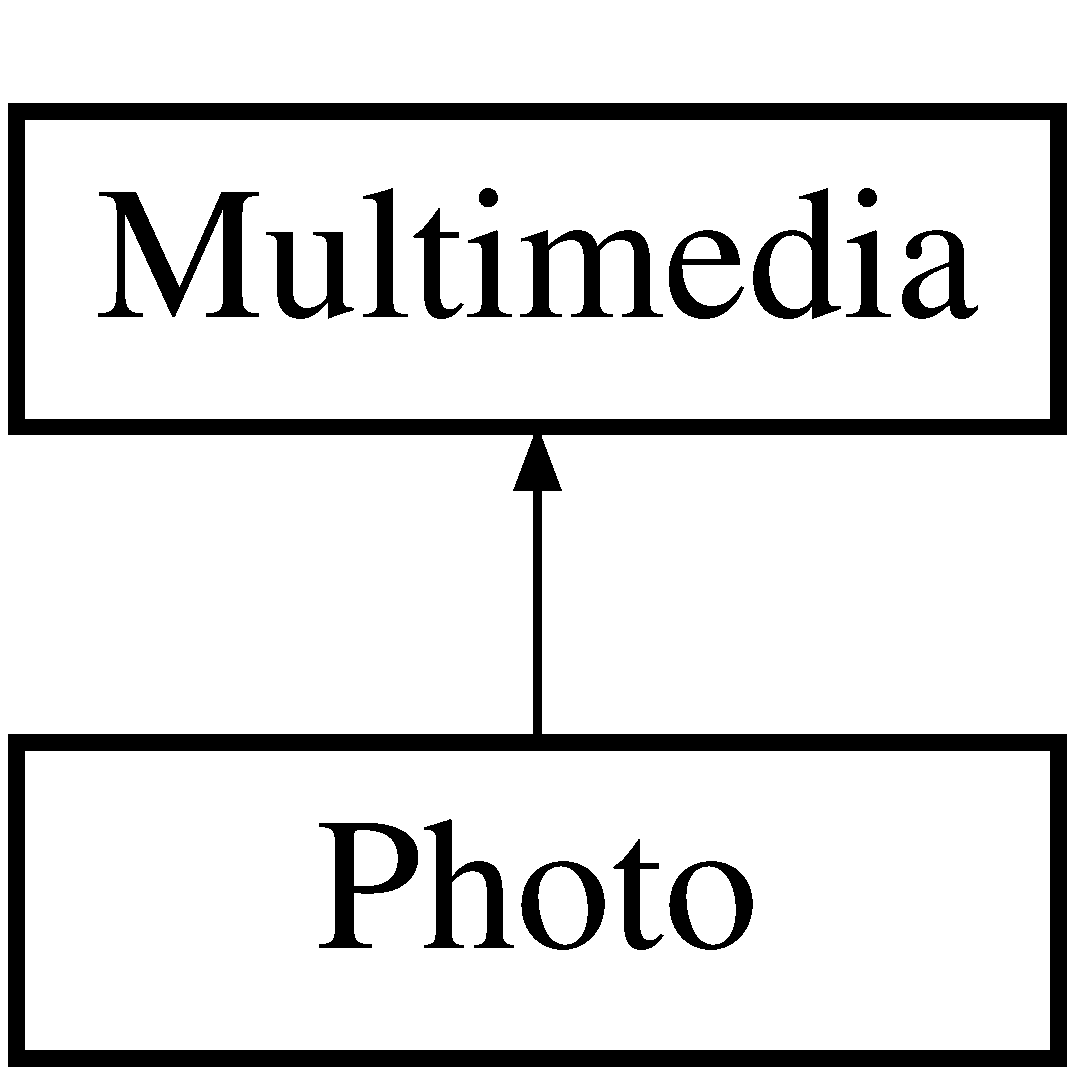
\includegraphics[height=2.000000cm]{class_photo}
\end{center}
\end{figure}
\subsection*{Classes}
\begin{DoxyCompactItemize}
\item 
class \hyperlink{class_photo_1_1_deleter_photo}{Deleter\-Photo}
\end{DoxyCompactItemize}
\subsection*{Public Member Functions}
\begin{DoxyCompactItemize}
\item 
virtual string \hyperlink{class_photo_a62050b13fc758cbb446f6170bf3dbc65}{get\-Place} (void) const 
\begin{DoxyCompactList}\small\item\em Place getter. \end{DoxyCompactList}\item 
\hypertarget{class_photo_a50a5f650f944ecb86d88855aad0bc492}{virtual void {\bfseries set\-Place} (string new\-Place)}\label{class_photo_a50a5f650f944ecb86d88855aad0bc492}

\item 
virtual string \hyperlink{class_photo_af63cb6130ed71a7f44d789fb3a5c7f01}{print} (void) const 
\begin{DoxyCompactList}\small\item\em Print description. \end{DoxyCompactList}\item 
\hypertarget{class_photo_a061bcd0e2002613bac15ce2e23543b0b}{virtual void \hyperlink{class_photo_a061bcd0e2002613bac15ce2e23543b0b}{play} (void) const }\label{class_photo_a061bcd0e2002613bac15ce2e23543b0b}

\begin{DoxyCompactList}\small\item\em Display the multimedia file on screen. \end{DoxyCompactList}\item 
virtual void \hyperlink{class_photo_a65c10b1d3dd17be4d478f7c3fb04ddd4}{write} (ostream \&stream) const 
\begin{DoxyCompactList}\small\item\em Serialize the multimedia object. \end{DoxyCompactList}\item 
virtual void \hyperlink{class_photo_a0c0ede69ed7502df226a95bbb62d7b40}{read} (istream \&stream)
\begin{DoxyCompactList}\small\item\em Read from a serialized object. \end{DoxyCompactList}\end{DoxyCompactItemize}
\subsection*{Protected Member Functions}
\begin{DoxyCompactItemize}
\item 
\hypertarget{class_photo_abb4bbd2c8364074c7605469378fcb059}{{\bfseries Photo} (const \hyperlink{class_photo}{Photo} \&)}\label{class_photo_abb4bbd2c8364074c7605469378fcb059}

\item 
\hyperlink{class_photo_a8824dbd5d05f0e39a258a4d73a61b17d}{Photo} (void)
\begin{DoxyCompactList}\small\item\em Default Constructor. \end{DoxyCompactList}\item 
\hyperlink{class_photo_a01773598a3f49a95c5b166534b35d7c5}{Photo} (string name, unsigned long date, string pathname, string place)
\begin{DoxyCompactList}\small\item\em Constructor. \end{DoxyCompactList}\item 
virtual \hyperlink{class_photo_a5ecb1bc1fde85af2f0405fa2d32a5a97}{$\sim$\-Photo} (void)
\begin{DoxyCompactList}\small\item\em Destructor. \end{DoxyCompactList}\item 
virtual \hyperlink{class_photo}{Photo} $\ast$ \hyperlink{class_photo_af8733ff93a45f0135076fcb731af56d7}{clone} (void) const 
\begin{DoxyCompactList}\small\item\em Clone the photo. \end{DoxyCompactList}\end{DoxyCompactItemize}
\subsection*{Friends}
\begin{DoxyCompactItemize}
\item 
\hypertarget{class_photo_a29a97f20d6ded769adf9ecc47158e24f}{class {\bfseries Multimedia\-Manager}}\label{class_photo_a29a97f20d6ded769adf9ecc47158e24f}

\item 
\hypertarget{class_photo_a06ed064be90eaa3ca877fb41f11dbe34}{class {\bfseries Deleter\-Photo}}\label{class_photo_a06ed064be90eaa3ca877fb41f11dbe34}

\end{DoxyCompactItemize}


\subsection{Detailed Description}
This class represents a photo file. 

\subsection{Constructor \& Destructor Documentation}
\hypertarget{class_photo_a8824dbd5d05f0e39a258a4d73a61b17d}{\index{Photo@{Photo}!Photo@{Photo}}
\index{Photo@{Photo}!Photo@{Photo}}
\subsubsection[{Photo}]{\setlength{\rightskip}{0pt plus 5cm}Photo\-::\-Photo (
\begin{DoxyParamCaption}
\item[{void}]{}
\end{DoxyParamCaption}
)\hspace{0.3cm}{\ttfamily [protected]}}}\label{class_photo_a8824dbd5d05f0e39a258a4d73a61b17d}


Default Constructor. 

Defaut constructor of a photo. \hypertarget{class_photo_a01773598a3f49a95c5b166534b35d7c5}{\index{Photo@{Photo}!Photo@{Photo}}
\index{Photo@{Photo}!Photo@{Photo}}
\subsubsection[{Photo}]{\setlength{\rightskip}{0pt plus 5cm}Photo\-::\-Photo (
\begin{DoxyParamCaption}
\item[{string}]{name, }
\item[{unsigned long}]{date, }
\item[{string}]{pathname, }
\item[{string}]{place}
\end{DoxyParamCaption}
)\hspace{0.3cm}{\ttfamily [protected]}}}\label{class_photo_a01773598a3f49a95c5b166534b35d7c5}


Constructor. 

Constructor of a photo.


\begin{DoxyParams}{Parameters}
{\em name} & \-: Name of the photo. \\
\hline
{\em date} & \-: Date when the file is added. \\
\hline
{\em pathname} & \-: Path to the photo. \\
\hline
{\em place} & \-: Place where the photo was taken. \\
\hline
\end{DoxyParams}
\hypertarget{class_photo_a5ecb1bc1fde85af2f0405fa2d32a5a97}{\index{Photo@{Photo}!$\sim$\-Photo@{$\sim$\-Photo}}
\index{$\sim$\-Photo@{$\sim$\-Photo}!Photo@{Photo}}
\subsubsection[{$\sim$\-Photo}]{\setlength{\rightskip}{0pt plus 5cm}Photo\-::$\sim$\-Photo (
\begin{DoxyParamCaption}
\item[{void}]{}
\end{DoxyParamCaption}
)\hspace{0.3cm}{\ttfamily [protected]}, {\ttfamily [virtual]}}}\label{class_photo_a5ecb1bc1fde85af2f0405fa2d32a5a97}


Destructor. 

Default destructor of this class. 

\subsection{Member Function Documentation}
\hypertarget{class_photo_af8733ff93a45f0135076fcb731af56d7}{\index{Photo@{Photo}!clone@{clone}}
\index{clone@{clone}!Photo@{Photo}}
\subsubsection[{clone}]{\setlength{\rightskip}{0pt plus 5cm}{\bf Photo} $\ast$ Photo\-::clone (
\begin{DoxyParamCaption}
\item[{void}]{}
\end{DoxyParamCaption}
) const\hspace{0.3cm}{\ttfamily [protected]}, {\ttfamily [virtual]}}}\label{class_photo_af8733ff93a45f0135076fcb731af56d7}


Clone the photo. 

\begin{DoxyReturn}{Returns}
Return a copy of the given photo. 
\end{DoxyReturn}


Implements \hyperlink{class_multimedia_a2955c15860b8310ee684d391e7b3386f}{Multimedia}.

\hypertarget{class_photo_a62050b13fc758cbb446f6170bf3dbc65}{\index{Photo@{Photo}!get\-Place@{get\-Place}}
\index{get\-Place@{get\-Place}!Photo@{Photo}}
\subsubsection[{get\-Place}]{\setlength{\rightskip}{0pt plus 5cm}string Photo\-::get\-Place (
\begin{DoxyParamCaption}
\item[{void}]{}
\end{DoxyParamCaption}
) const\hspace{0.3cm}{\ttfamily [virtual]}}}\label{class_photo_a62050b13fc758cbb446f6170bf3dbc65}


Place getter. 

Get the place where the photo was taken.

\begin{DoxyReturn}{Returns}
The place where the photo was taken. 
\end{DoxyReturn}
\hypertarget{class_photo_af63cb6130ed71a7f44d789fb3a5c7f01}{\index{Photo@{Photo}!print@{print}}
\index{print@{print}!Photo@{Photo}}
\subsubsection[{print}]{\setlength{\rightskip}{0pt plus 5cm}string Photo\-::print (
\begin{DoxyParamCaption}
\item[{void}]{}
\end{DoxyParamCaption}
) const\hspace{0.3cm}{\ttfamily [virtual]}}}\label{class_photo_af63cb6130ed71a7f44d789fb3a5c7f01}


Print description. 

Print the description of the file to the standard output \begin{DoxyReturn}{Returns}
Return a string which contains the file description. 
\end{DoxyReturn}


Reimplemented from \hyperlink{class_multimedia_a4960a7ffd22e90f74291ebf86eccf820}{Multimedia}.

\hypertarget{class_photo_a0c0ede69ed7502df226a95bbb62d7b40}{\index{Photo@{Photo}!read@{read}}
\index{read@{read}!Photo@{Photo}}
\subsubsection[{read}]{\setlength{\rightskip}{0pt plus 5cm}void Photo\-::read (
\begin{DoxyParamCaption}
\item[{istream \&}]{stream}
\end{DoxyParamCaption}
)\hspace{0.3cm}{\ttfamily [virtual]}}}\label{class_photo_a0c0ede69ed7502df226a95bbb62d7b40}


Read from a serialized object. 


\begin{DoxyParams}{Parameters}
{\em stream} & \-: the input stream where the object will be read. \\
\hline
\end{DoxyParams}


Implements \hyperlink{class_multimedia_ab686208e53fe8161bb86f7d37e01784c}{Multimedia}.

\hypertarget{class_photo_a65c10b1d3dd17be4d478f7c3fb04ddd4}{\index{Photo@{Photo}!write@{write}}
\index{write@{write}!Photo@{Photo}}
\subsubsection[{write}]{\setlength{\rightskip}{0pt plus 5cm}void Photo\-::write (
\begin{DoxyParamCaption}
\item[{ostream \&}]{stream}
\end{DoxyParamCaption}
) const\hspace{0.3cm}{\ttfamily [virtual]}}}\label{class_photo_a65c10b1d3dd17be4d478f7c3fb04ddd4}


Serialize the multimedia object. 


\begin{DoxyParams}{Parameters}
{\em stream} & \-: the output stream where the object will be written. \\
\hline
\end{DoxyParams}


Implements \hyperlink{class_multimedia_aa3c800e85ac5256ee8d1399d2ba33329}{Multimedia}.



The documentation for this class was generated from the following files\-:\begin{DoxyCompactItemize}
\item 
src/headers/photo.\-h\item 
src/photo.\-cpp\end{DoxyCompactItemize}

\hypertarget{class_pointable}{\section{Pointable Class Reference}
\label{class_pointable}\index{Pointable@{Pointable}}
}


{\ttfamily \#include $<$intrusive\-\_\-ptr.\-h$>$}

\subsection*{Public Member Functions}
\begin{DoxyCompactItemize}
\item 
\hypertarget{class_pointable_adc4da364054bdd4c4a9624f5dc190c8a}{{\bfseries Pointable} (const \hyperlink{class_pointable}{Pointable} \&)}\label{class_pointable_adc4da364054bdd4c4a9624f5dc190c8a}

\item 
\hypertarget{class_pointable_a8a7eb6956905e6e320ce97fa24f03b59}{\hyperlink{class_pointable}{Pointable} \& {\bfseries operator=} (const \hyperlink{class_pointable}{Pointable} \&)}\label{class_pointable_a8a7eb6956905e6e320ce97fa24f03b59}

\end{DoxyCompactItemize}
\subsection*{Friends}
\begin{DoxyCompactItemize}
\item 
\hypertarget{class_pointable_a9c08ce04af1d8cd2697b64990c51a5f4}{long {\bfseries intrusive\-\_\-ptr\-\_\-get\-\_\-count} (\hyperlink{class_pointable}{Pointable} $\ast$p)}\label{class_pointable_a9c08ce04af1d8cd2697b64990c51a5f4}

\item 
\hypertarget{class_pointable_a16ec5f964af06a93d6c7cfe0979ff672}{void {\bfseries intrusive\-\_\-ptr\-\_\-add\-\_\-ref} (\hyperlink{class_pointable}{Pointable} $\ast$p)}\label{class_pointable_a16ec5f964af06a93d6c7cfe0979ff672}

\item 
\hypertarget{class_pointable_aee25e5a73726af47eb078e2087eaee57}{void {\bfseries intrusive\-\_\-ptr\-\_\-release} (\hyperlink{class_pointable}{Pointable} $\ast$p)}\label{class_pointable_aee25e5a73726af47eb078e2087eaee57}

\end{DoxyCompactItemize}


\subsection{Detailed Description}
Generic base class for objects that can be pointed by an \hyperlink{classintrusive__ptr}{intrusive\-\_\-ptr}.
\begin{DoxyItemize}
\item \begin{DoxySeeAlso}{See Also}
\hyperlink{classintrusive__ptr}{intrusive\-\_\-ptr} for details
\end{DoxySeeAlso}

\item misc. checkings are performed if macro S\-M\-A\-R\-T\-\_\-\-P\-T\-R\-\_\-\-D\-E\-B\-U\-G is defined before including \hyperlink{intrusive__ptr_8h_source}{intrusive\-\_\-ptr.\-h}
\item debug messages are displayed on stderr if macros S\-M\-A\-R\-T\-\_\-\-P\-T\-R\-\_\-\-D\-E\-B\-U\-G and if S\-M\-A\-R\-T\-\_\-\-P\-T\-R\-\_\-\-D\-E\-B\-U\-G\-\_\-\-M\-E\-S\-S\-A\-G\-E\-S are both defined. 
\end{DoxyItemize}

The documentation for this class was generated from the following file\-:\begin{DoxyCompactItemize}
\item 
src/headers/intrusive\-\_\-ptr.\-h\end{DoxyCompactItemize}

\hypertarget{class_server_socket}{\section{Server\-Socket Class Reference}
\label{class_server_socket}\index{Server\-Socket@{Server\-Socket}}
}


{\ttfamily \#include $<$Socket.\-h$>$}

\subsection*{Public Member Functions}
\begin{DoxyCompactItemize}
\item 
\hyperlink{class_server_socket_a2b3098589541243241ca25495155186c}{Server\-Socket} ()
\item 
virtual \hyperlink{class_socket}{Socket} $\ast$ \hyperlink{class_server_socket_accc3d56d42aa50a5f3c920cf0b26959b}{accept} ()
\item 
virtual int \hyperlink{class_server_socket_ad5281fe6c005bca007a9a758bd612481}{bind} (int port, int backlog=50)
\item 
\hypertarget{class_server_socket_a3eac6d5571bb092622d328dbda2de2cf}{virtual int \hyperlink{class_server_socket_a3eac6d5571bb092622d328dbda2de2cf}{close} ()}\label{class_server_socket_a3eac6d5571bb092622d328dbda2de2cf}

\begin{DoxyCompactList}\small\item\em Closes the socket. \end{DoxyCompactList}\item 
\hypertarget{class_server_socket_a73a32b4697d3ff2bc9a68700f06e4dfb}{int \hyperlink{class_server_socket_a73a32b4697d3ff2bc9a68700f06e4dfb}{get\-File\-Descriptor} () const }\label{class_server_socket_a73a32b4697d3ff2bc9a68700f06e4dfb}

\begin{DoxyCompactList}\small\item\em Returns the file descriptor of the socket. \end{DoxyCompactList}\item 
void \hyperlink{class_server_socket_afe81d7c30d1e963e6a043b868560dbbd}{handle\-Sig\-Pipe} (void($\ast$function)(int signal))
\item 
void \hyperlink{class_server_socket_ac159a12414df54dfef149a8de6aacb20}{ignore\-Sig\-Pipe} ()
\begin{DoxyCompactList}\small\item\em Ignore S\-I\-G\-P\-I\-P\-E signals (. \end{DoxyCompactList}\item 
int \hyperlink{class_server_socket_a7ad8a5581c52046e641b32d96eb23406}{get\-Option} (int level, int optname, void $\ast$optval, socklen\-\_\-t $\ast$optlen)
\item 
int \hyperlink{class_server_socket_ad69fa5c5891f028192a291044b9191e2}{set\-Option} (int level, int optname, const void $\ast$optval, socklen\-\_\-t optlen)
\item 
\hypertarget{class_server_socket_ab34154bc6114c638ae02f5e018121099}{int \hyperlink{class_server_socket_ab34154bc6114c638ae02f5e018121099}{set\-Receive\-Buffer\-Size} (int size)}\label{class_server_socket_ab34154bc6114c638ae02f5e018121099}

\begin{DoxyCompactList}\small\item\em Sets the S\-O\-\_\-\-R\-C\-V\-B\-U\-F option to the specified value. \end{DoxyCompactList}\item 
\hypertarget{class_server_socket_ae60d7cc31ad535e5d3cac42e38b8ec98}{int \hyperlink{class_server_socket_ae60d7cc31ad535e5d3cac42e38b8ec98}{set\-Reuse\-Address} (bool)}\label{class_server_socket_ae60d7cc31ad535e5d3cac42e38b8ec98}

\begin{DoxyCompactList}\small\item\em Enables/disables the S\-O\-\_\-\-R\-E\-U\-S\-E\-A\-D\-D\-R socket option. \end{DoxyCompactList}\item 
\hypertarget{class_server_socket_aedb9144c9c375fcb14ac47bcb9d2eb17}{int \hyperlink{class_server_socket_aedb9144c9c375fcb14ac47bcb9d2eb17}{set\-So\-Timeout} (int timeout)}\label{class_server_socket_aedb9144c9c375fcb14ac47bcb9d2eb17}

\begin{DoxyCompactList}\small\item\em Enables/disables S\-O\-\_\-\-T\-I\-M\-E\-O\-U\-T with the specified timeout (in milliseconds). \end{DoxyCompactList}\item 
\hypertarget{class_server_socket_a9e5e1ee852ba26156c757a0086b780fe}{int \hyperlink{class_server_socket_a9e5e1ee852ba26156c757a0086b780fe}{set\-Tcp\-No\-Delay} (bool)}\label{class_server_socket_a9e5e1ee852ba26156c757a0086b780fe}

\begin{DoxyCompactList}\small\item\em Turns on/off T\-C\-P coalescence (useful in some cases to avoid delays). \end{DoxyCompactList}\end{DoxyCompactItemize}


\subsection{Detailed Description}
T\-C\-P/\-I\-P \hyperlink{class_socket}{Socket} Server. Note\-: this class supports A\-F\-\_\-\-I\-N\-E\-T connections following the I\-Pv4 Internet protocol. Other families, such as A\-F\-\_\-\-I\-N\-E\-T6 or A\-F\-\_\-\-U\-N\-I\-X are not yet supported. 

\subsection{Constructor \& Destructor Documentation}
\hypertarget{class_server_socket_a2b3098589541243241ca25495155186c}{\index{Server\-Socket@{Server\-Socket}!Server\-Socket@{Server\-Socket}}
\index{Server\-Socket@{Server\-Socket}!ServerSocket@{Server\-Socket}}
\subsubsection[{Server\-Socket}]{\setlength{\rightskip}{0pt plus 5cm}Server\-Socket\-::\-Server\-Socket (
\begin{DoxyParamCaption}
{}
\end{DoxyParamCaption}
)}}\label{class_server_socket_a2b3098589541243241ca25495155186c}
creates a new \hyperlink{class_server_socket}{Server\-Socket}. Creates a listening A\-F\-\_\-\-I\-N\-E\-T socket (using the I\-Pv4 Internet protocol) that waits for connection requests by T\-C\-P/\-I\-P (S\-O\-C\-K\-\_\-\-S\-T\-R\-E\-A\-M) client sockets. 

\subsection{Member Function Documentation}
\hypertarget{class_server_socket_accc3d56d42aa50a5f3c920cf0b26959b}{\index{Server\-Socket@{Server\-Socket}!accept@{accept}}
\index{accept@{accept}!ServerSocket@{Server\-Socket}}
\subsubsection[{accept}]{\setlength{\rightskip}{0pt plus 5cm}{\bf Socket} $\ast$ Server\-Socket\-::accept (
\begin{DoxyParamCaption}
{}
\end{DoxyParamCaption}
)\hspace{0.3cm}{\ttfamily [virtual]}}}\label{class_server_socket_accc3d56d42aa50a5f3c920cf0b26959b}
Accepts a new connection request and returns the corresponding socket. By default, this function blocks the caller until a connection is present \begin{DoxyReturn}{Returns}
Returns the new \hyperlink{class_socket}{Socket} or N\-U\-L\-L on error 
\end{DoxyReturn}
\hypertarget{class_server_socket_ad5281fe6c005bca007a9a758bd612481}{\index{Server\-Socket@{Server\-Socket}!bind@{bind}}
\index{bind@{bind}!ServerSocket@{Server\-Socket}}
\subsubsection[{bind}]{\setlength{\rightskip}{0pt plus 5cm}int Server\-Socket\-::bind (
\begin{DoxyParamCaption}
\item[{int}]{port, }
\item[{int}]{backlog = {\ttfamily 50}}
\end{DoxyParamCaption}
)\hspace{0.3cm}{\ttfamily [virtual]}}}\label{class_server_socket_ad5281fe6c005bca007a9a758bd612481}
Assigns the socket to the local address. \begin{DoxyReturn}{Returns}
0 on success or a negative value on error which is one of \hyperlink{class_socket_a9f68308228badcdd299cd83e62e36976}{Socket\-::\-Errors} 
\end{DoxyReturn}
\hypertarget{class_server_socket_a7ad8a5581c52046e641b32d96eb23406}{\index{Server\-Socket@{Server\-Socket}!get\-Option@{get\-Option}}
\index{get\-Option@{get\-Option}!ServerSocket@{Server\-Socket}}
\subsubsection[{get\-Option}]{\setlength{\rightskip}{0pt plus 5cm}int Server\-Socket\-::get\-Option (
\begin{DoxyParamCaption}
\item[{int}]{level, }
\item[{int}]{optname, }
\item[{void $\ast$}]{optval, }
\item[{socklen\-\_\-t $\ast$}]{optlen}
\end{DoxyParamCaption}
)}}\label{class_server_socket_a7ad8a5581c52046e641b32d96eb23406}
Gets socket options. Same arguments and effect as the getsockopt() system call. \begin{DoxyReturn}{Returns}
On success, zero is returned. On error, -\/1 is returned. 
\end{DoxyReturn}
\hypertarget{class_server_socket_afe81d7c30d1e963e6a043b868560dbbd}{\index{Server\-Socket@{Server\-Socket}!handle\-Sig\-Pipe@{handle\-Sig\-Pipe}}
\index{handle\-Sig\-Pipe@{handle\-Sig\-Pipe}!ServerSocket@{Server\-Socket}}
\subsubsection[{handle\-Sig\-Pipe}]{\setlength{\rightskip}{0pt plus 5cm}void Server\-Socket\-::handle\-Sig\-Pipe (
\begin{DoxyParamCaption}
\item[{void($\ast$)(int signal)}]{function}
\end{DoxyParamCaption}
)}}\label{class_server_socket_afe81d7c30d1e963e6a043b868560dbbd}
Handle S\-I\-G\-P\-I\-P\-E signals. Sockets may abort programs by throwing a S\-I\-G\-P\-I\-P\-E signal. The function given as an argument will be called instead of aborting the program.  \hyperlink{class_server_socket_ac159a12414df54dfef149a8de6aacb20}{ignore\-Sig\-Pipe()} \hypertarget{class_server_socket_ac159a12414df54dfef149a8de6aacb20}{\index{Server\-Socket@{Server\-Socket}!ignore\-Sig\-Pipe@{ignore\-Sig\-Pipe}}
\index{ignore\-Sig\-Pipe@{ignore\-Sig\-Pipe}!ServerSocket@{Server\-Socket}}
\subsubsection[{ignore\-Sig\-Pipe}]{\setlength{\rightskip}{0pt plus 5cm}void Server\-Socket\-::ignore\-Sig\-Pipe (
\begin{DoxyParamCaption}
{}
\end{DoxyParamCaption}
)}}\label{class_server_socket_ac159a12414df54dfef149a8de6aacb20}


Ignore S\-I\-G\-P\-I\-P\-E signals (. 

\begin{DoxySeeAlso}{See Also}
\hyperlink{class_server_socket_afe81d7c30d1e963e6a043b868560dbbd}{handle\-Sig\-Pipe()}). 
\end{DoxySeeAlso}
\hypertarget{class_server_socket_ad69fa5c5891f028192a291044b9191e2}{\index{Server\-Socket@{Server\-Socket}!set\-Option@{set\-Option}}
\index{set\-Option@{set\-Option}!ServerSocket@{Server\-Socket}}
\subsubsection[{set\-Option}]{\setlength{\rightskip}{0pt plus 5cm}int Server\-Socket\-::set\-Option (
\begin{DoxyParamCaption}
\item[{int}]{level, }
\item[{int}]{optname, }
\item[{const void $\ast$}]{optval, }
\item[{socklen\-\_\-t}]{optlen}
\end{DoxyParamCaption}
)}}\label{class_server_socket_ad69fa5c5891f028192a291044b9191e2}
Sets socket options. Same arguments and effect as the setsockopt() system call. \begin{DoxyReturn}{Returns}
On success, zero is returned. On error, -\/1 is returned.  helper functions \hyperlink{class_server_socket_ae60d7cc31ad535e5d3cac42e38b8ec98}{set\-Reuse\-Address()}, \hyperlink{class_server_socket_a9e5e1ee852ba26156c757a0086b780fe}{set\-Tcp\-No\-Delay()}, etc. 
\end{DoxyReturn}


The documentation for this class was generated from the following files\-:\begin{DoxyCompactItemize}
\item 
src/headers/Socket.\-h\item 
src/\-Server/Socket.\-cpp\end{DoxyCompactItemize}

\hypertarget{class_socket}{\section{Socket Class Reference}
\label{class_socket}\index{Socket@{Socket}}
}


{\ttfamily \#include $<$Socket.\-h$>$}

\subsection*{Public Types}
\begin{DoxyCompactItemize}
\item 
enum \hyperlink{class_socket_a9f68308228badcdd299cd83e62e36976}{Errors} \{ {\bfseries F\-A\-I\-L\-E\-D} = -\/1, 
{\bfseries I\-N\-V\-A\-L\-I\-D\-\_\-\-S\-O\-C\-K\-E\-T} = -\/2, 
{\bfseries U\-N\-K\-N\-O\-W\-N\-\_\-\-H\-O\-S\-T} = -\/3
 \}
\end{DoxyCompactItemize}
\subsection*{Public Member Functions}
\begin{DoxyCompactItemize}
\item 
\hyperlink{class_socket_acd3cb39bc957be2f34c91b9e262e1cec}{Socket} (int type=S\-O\-C\-K\-\_\-\-S\-T\-R\-E\-A\-M)
\item 
\hypertarget{class_socket_a14170941ba1aaa3263f3e8dd3f85e24f}{\hyperlink{class_socket_a14170941ba1aaa3263f3e8dd3f85e24f}{Socket} (int type, int sockfd)}\label{class_socket_a14170941ba1aaa3263f3e8dd3f85e24f}

\begin{DoxyCompactList}\small\item\em Creates a socket object from an existing socket file descriptor. \end{DoxyCompactList}\item 
virtual \hyperlink{class_socket_aeac4eb6379a543d38ed88977d3b6630a}{$\sim$\-Socket} ()
\item 
virtual int \hyperlink{class_socket_a019fdc04fe2afd7aecd612469be32467}{bind} (int port=0)
\item 
virtual int \hyperlink{class_socket_a8f014a801fb3e61bbee00b84c06f2330}{bind} (const std\-::string \&host, int port)
\item 
virtual int \hyperlink{class_socket_aac9588a21bb2c52ff8246272cf36834a}{connect} (const std\-::string \&remote\-Host, int port)
\item 
virtual int \hyperlink{class_socket_aef06605c6725958004116983f1a2051f}{close} ()
\item 
\hypertarget{class_socket_a6b4449d6b454bdb4a3a809976a3c2e41}{int \hyperlink{class_socket_a6b4449d6b454bdb4a3a809976a3c2e41}{get\-File\-Descriptor} () const }\label{class_socket_a6b4449d6b454bdb4a3a809976a3c2e41}

\begin{DoxyCompactList}\small\item\em Returns the file descriptor of the socket. \end{DoxyCompactList}\item 
ssize\-\_\-t \hyperlink{class_socket_a9275eacdb64056a53cf4b9cf54cd2f1a}{send} (const void $\ast$buf, size\-\_\-t len, int flags=0)
\item 
ssize\-\_\-t \hyperlink{class_socket_aa5e98b6f2c4e26fcf90d71c8386fc09d}{receive} (void $\ast$buf, size\-\_\-t len, int flags=0)
\item 
ssize\-\_\-t \hyperlink{class_socket_ac75e3ac80b7e6ae1bdce58c1c4e2b56a}{send\-To} (const void $\ast$buf, size\-\_\-t len, int flags, const struct sockaddr $\ast$dest\-\_\-addr, socklen\-\_\-t addrlen)
\item 
ssize\-\_\-t \hyperlink{class_socket_a7cca10ce2a21e0648850e55a878f51b2}{receive\-From} (void $\ast$buf, size\-\_\-t len, int flags, struct sockaddr $\ast$src\-\_\-addr, socklen\-\_\-t $\ast$addrlen)
\item 
\hypertarget{class_socket_a417b47af24de10184192de00d9112589}{virtual void \hyperlink{class_socket_a417b47af24de10184192de00d9112589}{shutdown\-Input} ()}\label{class_socket_a417b47af24de10184192de00d9112589}

\begin{DoxyCompactList}\small\item\em Disables further receive operations. \end{DoxyCompactList}\item 
\hypertarget{class_socket_a650128aee2581e6695c6812d8afe14b5}{virtual void \hyperlink{class_socket_a650128aee2581e6695c6812d8afe14b5}{shutdown\-Output} ()}\label{class_socket_a650128aee2581e6695c6812d8afe14b5}

\begin{DoxyCompactList}\small\item\em Disables further send operations. \end{DoxyCompactList}\item 
virtual int \hyperlink{class_socket_adc250da2f4f1e813850b83cc0be04fa2}{get\-Option} (int level, int optname, void $\ast$optval, socklen\-\_\-t $\ast$optlen)
\item 
virtual int \hyperlink{class_socket_aede9a4b4ef00a7169f8eec1e75f1796d}{set\-Option} (int level, int optname, const void $\ast$optval, socklen\-\_\-t optlen)
\item 
\hypertarget{class_socket_a06ff0dd6837c9f51948df655fc2713cd}{int \hyperlink{class_socket_a06ff0dd6837c9f51948df655fc2713cd}{set\-Receive\-Buffer\-Size} (int size)}\label{class_socket_a06ff0dd6837c9f51948df655fc2713cd}

\begin{DoxyCompactList}\small\item\em Sets the S\-O\-\_\-\-R\-C\-V\-B\-U\-F option to the specified value. \end{DoxyCompactList}\item 
\hypertarget{class_socket_ab02b997fa7e251d596116e95c9ccaf97}{int \hyperlink{class_socket_ab02b997fa7e251d596116e95c9ccaf97}{set\-Reuse\-Address} (bool)}\label{class_socket_ab02b997fa7e251d596116e95c9ccaf97}

\begin{DoxyCompactList}\small\item\em Enables/disables the S\-O\-\_\-\-R\-E\-U\-S\-E\-A\-D\-D\-R socket option. \end{DoxyCompactList}\item 
\hypertarget{class_socket_afc49ad6cc259a0006ca13bb22fdd7383}{int \hyperlink{class_socket_afc49ad6cc259a0006ca13bb22fdd7383}{set\-Send\-Buffer\-Size} (int size)}\label{class_socket_afc49ad6cc259a0006ca13bb22fdd7383}

\begin{DoxyCompactList}\small\item\em Sets the S\-O\-\_\-\-S\-N\-D\-B\-U\-F option to the specified value. \end{DoxyCompactList}\item 
\hypertarget{class_socket_a41cc1caae51e3e83e16ce2c20689ed03}{int \hyperlink{class_socket_a41cc1caae51e3e83e16ce2c20689ed03}{set\-So\-Linger} (bool, int linger)}\label{class_socket_a41cc1caae51e3e83e16ce2c20689ed03}

\begin{DoxyCompactList}\small\item\em Enables/disables S\-O\-\_\-\-L\-I\-N\-G\-E\-R with the specified linger time in seconds. \end{DoxyCompactList}\item 
\hypertarget{class_socket_ad65a22ec40902e2c0a98c5d4ac885f99}{int \hyperlink{class_socket_ad65a22ec40902e2c0a98c5d4ac885f99}{set\-So\-Timeout} (int timeout)}\label{class_socket_ad65a22ec40902e2c0a98c5d4ac885f99}

\begin{DoxyCompactList}\small\item\em Enables/disables S\-O\-\_\-\-T\-I\-M\-E\-O\-U\-T with the specified timeout (in milliseconds). \end{DoxyCompactList}\item 
\hypertarget{class_socket_a7bc0110f3bedbb18f26b05ece01553fa}{int \hyperlink{class_socket_a7bc0110f3bedbb18f26b05ece01553fa}{set\-Tcp\-No\-Delay} (bool)}\label{class_socket_a7bc0110f3bedbb18f26b05ece01553fa}

\begin{DoxyCompactList}\small\item\em Turns on/off T\-C\-P coalescence (useful in some cases to avoid delays). \end{DoxyCompactList}\item 
\hypertarget{class_socket_ae098ebe2d34fac9947260f517ee8de04}{virtual int \hyperlink{class_socket_ae098ebe2d34fac9947260f517ee8de04}{set\-Local\-Address} (struct sockaddr\-\_\-in \&addr, int port)}\label{class_socket_ae098ebe2d34fac9947260f517ee8de04}

\begin{DoxyCompactList}\small\item\em Initializes a local I\-N\-E\-T4 address, returns 0 on success, -\/1 otherwise. \end{DoxyCompactList}\item 
\hypertarget{class_socket_aec683b1b0104aeae9fc2cfdbb6b70e9f}{virtual int \hyperlink{class_socket_aec683b1b0104aeae9fc2cfdbb6b70e9f}{set\-Address} (struct sockaddr\-\_\-in \&addr, const std\-::string \&host, int port)}\label{class_socket_aec683b1b0104aeae9fc2cfdbb6b70e9f}

\begin{DoxyCompactList}\small\item\em Initializes a remote I\-N\-E\-T4 address, returns 0 on success, -\/1 otherwise. \end{DoxyCompactList}\end{DoxyCompactItemize}
\subsection*{Friends}
\begin{DoxyCompactItemize}
\item 
\hypertarget{class_socket_a11a8bb11feaafab939278a8285afa567}{class {\bfseries Server\-Socket}}\label{class_socket_a11a8bb11feaafab939278a8285afa567}

\end{DoxyCompactItemize}


\subsection{Detailed Description}
T\-C\-P/\-I\-P or U\-D\-P Datagram \hyperlink{class_socket}{Socket}. Note\-: this class supports A\-F\-\_\-\-I\-N\-E\-T connections following the I\-Pv4 Internet protocol. Other families, such as A\-F\-\_\-\-I\-N\-E\-T6 or A\-F\-\_\-\-U\-N\-I\-X are not yet supported. 

\subsection{Member Enumeration Documentation}
\hypertarget{class_socket_a9f68308228badcdd299cd83e62e36976}{\index{Socket@{Socket}!Errors@{Errors}}
\index{Errors@{Errors}!Socket@{Socket}}
\subsubsection[{Errors}]{\setlength{\rightskip}{0pt plus 5cm}enum {\bf Socket\-::\-Errors}}}\label{class_socket_a9f68308228badcdd299cd83e62e36976}
\hyperlink{class_socket}{Socket} errors.
\begin{DoxyItemize}
\item Socket\-::\-F\-A\-I\-L\-E\-D (-\/1)\-: could not connect, could not bind, etc.
\item Socket\-::\-I\-N\-V\-A\-L\-I\-D\-\_\-\-S\-O\-C\-K\-E\-T (-\/2)\-: wrong socket type.
\item Socket\-::\-U\-N\-K\-N\-O\-W\-N\-\_\-\-H\-O\-S\-T (-\/3)\-: could not reach host 
\end{DoxyItemize}

\subsection{Constructor \& Destructor Documentation}
\hypertarget{class_socket_acd3cb39bc957be2f34c91b9e262e1cec}{\index{Socket@{Socket}!Socket@{Socket}}
\index{Socket@{Socket}!Socket@{Socket}}
\subsubsection[{Socket}]{\setlength{\rightskip}{0pt plus 5cm}Socket\-::\-Socket (
\begin{DoxyParamCaption}
\item[{int}]{type = {\ttfamily SOCK\-\_\-STREAM}}
\end{DoxyParamCaption}
)}}\label{class_socket_acd3cb39bc957be2f34c91b9e262e1cec}
Creates a new socket. Creates a A\-F\-\_\-\-I\-N\-E\-T socket using the I\-Pv4 Internet protocol. Type can be\-:
\begin{DoxyItemize}
\item S\-O\-C\-K\-\_\-\-S\-T\-R\-E\-A\-M (the default) for T\-C\-P/\-I\-P connected stream sockets
\item S\-O\-C\-K\-\_\-\-D\-G\-R\-A\-M for U\-D\-P datagram sockets 
\end{DoxyItemize}\hypertarget{class_socket_aeac4eb6379a543d38ed88977d3b6630a}{\index{Socket@{Socket}!$\sim$\-Socket@{$\sim$\-Socket}}
\index{$\sim$\-Socket@{$\sim$\-Socket}!Socket@{Socket}}
\subsubsection[{$\sim$\-Socket}]{\setlength{\rightskip}{0pt plus 5cm}Socket\-::$\sim$\-Socket (
\begin{DoxyParamCaption}
{}
\end{DoxyParamCaption}
)\hspace{0.3cm}{\ttfamily [virtual]}}}\label{class_socket_aeac4eb6379a543d38ed88977d3b6630a}
Destructor. Closes the socket. 

\subsection{Member Function Documentation}
\hypertarget{class_socket_a019fdc04fe2afd7aecd612469be32467}{\index{Socket@{Socket}!bind@{bind}}
\index{bind@{bind}!Socket@{Socket}}
\subsubsection[{bind}]{\setlength{\rightskip}{0pt plus 5cm}int Socket\-::bind (
\begin{DoxyParamCaption}
\item[{int}]{port = {\ttfamily 0}}
\end{DoxyParamCaption}
)\hspace{0.3cm}{\ttfamily [virtual]}}}\label{class_socket_a019fdc04fe2afd7aecd612469be32467}
Assigns the socket to the local address. \begin{DoxyReturn}{Returns}
0 on success or a negative value on error which is one of \hyperlink{class_socket_a9f68308228badcdd299cd83e62e36976}{Socket\-::\-Errors} 
\end{DoxyReturn}
\hypertarget{class_socket_a8f014a801fb3e61bbee00b84c06f2330}{\index{Socket@{Socket}!bind@{bind}}
\index{bind@{bind}!Socket@{Socket}}
\subsubsection[{bind}]{\setlength{\rightskip}{0pt plus 5cm}virtual int Socket\-::bind (
\begin{DoxyParamCaption}
\item[{const std\-::string \&}]{host, }
\item[{int}]{port}
\end{DoxyParamCaption}
)\hspace{0.3cm}{\ttfamily [virtual]}}}\label{class_socket_a8f014a801fb3e61bbee00b84c06f2330}
Assigns the socket to this address. \begin{DoxyReturn}{Returns}
0 on success or a negative value on error which is one of \hyperlink{class_socket_a9f68308228badcdd299cd83e62e36976}{Socket\-::\-Errors} 
\end{DoxyReturn}
\hypertarget{class_socket_aef06605c6725958004116983f1a2051f}{\index{Socket@{Socket}!close@{close}}
\index{close@{close}!Socket@{Socket}}
\subsubsection[{close}]{\setlength{\rightskip}{0pt plus 5cm}int Socket\-::close (
\begin{DoxyParamCaption}
{}
\end{DoxyParamCaption}
)\hspace{0.3cm}{\ttfamily [virtual]}}}\label{class_socket_aef06605c6725958004116983f1a2051f}
Closes the socket. \begin{DoxyReturn}{Returns}
0 on success and -\/1 on error. 
\end{DoxyReturn}
\hypertarget{class_socket_aac9588a21bb2c52ff8246272cf36834a}{\index{Socket@{Socket}!connect@{connect}}
\index{connect@{connect}!Socket@{Socket}}
\subsubsection[{connect}]{\setlength{\rightskip}{0pt plus 5cm}int Socket\-::connect (
\begin{DoxyParamCaption}
\item[{const std\-::string \&}]{remote\-Host, }
\item[{int}]{port}
\end{DoxyParamCaption}
)\hspace{0.3cm}{\ttfamily [virtual]}}}\label{class_socket_aac9588a21bb2c52ff8246272cf36834a}
Connects the socket to a server socket. \begin{DoxyReturn}{Returns}
0 on success or a negative value on error which is one of \hyperlink{class_socket_a9f68308228badcdd299cd83e62e36976}{Socket\-::\-Errors} 
\end{DoxyReturn}
\begin{DoxySeeAlso}{See Also}
\hyperlink{class_server_socket}{Server\-Socket}. 
\end{DoxySeeAlso}
\hypertarget{class_socket_adc250da2f4f1e813850b83cc0be04fa2}{\index{Socket@{Socket}!get\-Option@{get\-Option}}
\index{get\-Option@{get\-Option}!Socket@{Socket}}
\subsubsection[{get\-Option}]{\setlength{\rightskip}{0pt plus 5cm}int Socket\-::get\-Option (
\begin{DoxyParamCaption}
\item[{int}]{level, }
\item[{int}]{optname, }
\item[{void $\ast$}]{optval, }
\item[{socklen\-\_\-t $\ast$}]{optlen}
\end{DoxyParamCaption}
)\hspace{0.3cm}{\ttfamily [virtual]}}}\label{class_socket_adc250da2f4f1e813850b83cc0be04fa2}
Gets socket options. \begin{DoxySeeAlso}{See Also}
the getsockopt() system call. 
\end{DoxySeeAlso}
\begin{DoxyReturn}{Returns}
0 on success and -\/1 on error. 
\end{DoxyReturn}
\hypertarget{class_socket_aa5e98b6f2c4e26fcf90d71c8386fc09d}{\index{Socket@{Socket}!receive@{receive}}
\index{receive@{receive}!Socket@{Socket}}
\subsubsection[{receive}]{\setlength{\rightskip}{0pt plus 5cm}ssize\-\_\-t Socket\-::receive (
\begin{DoxyParamCaption}
\item[{void $\ast$}]{buf, }
\item[{size\-\_\-t}]{len, }
\item[{int}]{flags = {\ttfamily 0}}
\end{DoxyParamCaption}
)\hspace{0.3cm}{\ttfamily [inline]}}}\label{class_socket_aa5e98b6f2c4e26fcf90d71c8386fc09d}
Receives data from a connected socket. Reads {\itshape at most} {\itshape len} bytes from a connected (i.\-e. S\-O\-C\-K\-\_\-\-S\-T\-R\-E\-A\-M) socket. By default, this function blocks the caller until data is present (\begin{DoxySeeAlso}{See Also}
recv()), except if end-\/of-\/stream is reached (\hyperlink{class_socket_a650128aee2581e6695c6812d8afe14b5}{shutdown\-Output()} was called on the other side) or an error occurs. 
\end{DoxySeeAlso}
\begin{DoxyReturn}{Returns}
the number of bytes received, 0 at end-\/of-\/stream, -\/1 in case of an error. 
\end{DoxyReturn}
\begin{DoxyNote}{Note}
that that connected sockets do not preserve record boundaries (
\end{DoxyNote}
\begin{DoxySeeAlso}{See Also}
\hyperlink{class_socket_buffer}{Socket\-Buffer}). 

\hyperlink{class_socket_buffer}{Socket\-Buffer} to preserve record boundaries. 

the recv() system call for low level details. 
\end{DoxySeeAlso}
\hypertarget{class_socket_a7cca10ce2a21e0648850e55a878f51b2}{\index{Socket@{Socket}!receive\-From@{receive\-From}}
\index{receive\-From@{receive\-From}!Socket@{Socket}}
\subsubsection[{receive\-From}]{\setlength{\rightskip}{0pt plus 5cm}ssize\-\_\-t Socket\-::receive\-From (
\begin{DoxyParamCaption}
\item[{void $\ast$}]{buf, }
\item[{size\-\_\-t}]{len, }
\item[{int}]{flags, }
\item[{struct sockaddr $\ast$}]{src\-\_\-addr, }
\item[{socklen\-\_\-t $\ast$}]{addrlen}
\end{DoxyParamCaption}
)\hspace{0.3cm}{\ttfamily [inline]}}}\label{class_socket_a7cca10ce2a21e0648850e55a878f51b2}
Receives data from datagram socket. Reads at most {\itshape len} bytes from a datagram (i.\-e. S\-O\-C\-K\-\_\-\-D\-G\-R\-A\-M) socket. By default, this function blocks the caller until data is present (\begin{DoxySeeAlso}{See Also}
recv()). 
\end{DoxySeeAlso}
\begin{DoxyReturn}{Returns}
the number of bytes received, -\/1 in case of an error, 0 at end-\/of-\/stream (e.\-g. if \hyperlink{class_socket_a650128aee2581e6695c6812d8afe14b5}{shutdown\-Output()} was called on the other side). 
\end{DoxyReturn}
\begin{DoxySeeAlso}{See Also}
the recvfrom() system call for low level details. 
\end{DoxySeeAlso}
\hypertarget{class_socket_a9275eacdb64056a53cf4b9cf54cd2f1a}{\index{Socket@{Socket}!send@{send}}
\index{send@{send}!Socket@{Socket}}
\subsubsection[{send}]{\setlength{\rightskip}{0pt plus 5cm}ssize\-\_\-t Socket\-::send (
\begin{DoxyParamCaption}
\item[{const void $\ast$}]{buf, }
\item[{size\-\_\-t}]{len, }
\item[{int}]{flags = {\ttfamily 0}}
\end{DoxyParamCaption}
)\hspace{0.3cm}{\ttfamily [inline]}}}\label{class_socket_a9275eacdb64056a53cf4b9cf54cd2f1a}
Sends data to a connected socket. Sends {\itshape len} bytes to a connected (i.\-e. S\-O\-C\-K\-\_\-\-S\-T\-R\-E\-A\-M) socket. \begin{DoxyReturn}{Returns}
the number of bytes sent or -\/1 in case of an error. 
\end{DoxyReturn}
\begin{DoxyNote}{Note}
that that connected sockets do not preserve record boundaries (
\end{DoxyNote}
\begin{DoxySeeAlso}{See Also}
\hyperlink{class_socket_buffer}{Socket\-Buffer}). 

\hyperlink{class_socket_buffer}{Socket\-Buffer} to preserve record boundaries. 

the \hyperlink{class_socket_a9275eacdb64056a53cf4b9cf54cd2f1a}{send()} system call for low level details. 
\end{DoxySeeAlso}
\hypertarget{class_socket_ac75e3ac80b7e6ae1bdce58c1c4e2b56a}{\index{Socket@{Socket}!send\-To@{send\-To}}
\index{send\-To@{send\-To}!Socket@{Socket}}
\subsubsection[{send\-To}]{\setlength{\rightskip}{0pt plus 5cm}ssize\-\_\-t Socket\-::send\-To (
\begin{DoxyParamCaption}
\item[{const void $\ast$}]{buf, }
\item[{size\-\_\-t}]{len, }
\item[{int}]{flags, }
\item[{const struct sockaddr $\ast$}]{dest\-\_\-addr, }
\item[{socklen\-\_\-t}]{addrlen}
\end{DoxyParamCaption}
)\hspace{0.3cm}{\ttfamily [inline]}}}\label{class_socket_ac75e3ac80b7e6ae1bdce58c1c4e2b56a}
Sends data to a datagram socket. Sends {\itshape len} bytes to a datagram (i.\-e. S\-O\-C\-K\-\_\-\-D\-G\-R\-A\-M) socket. \begin{DoxyReturn}{Returns}
the number of bytes sent or -\/1 in case of an error. 
\end{DoxyReturn}
\begin{DoxySeeAlso}{See Also}
the sendto() system call for low level details. 
\end{DoxySeeAlso}
\hypertarget{class_socket_aede9a4b4ef00a7169f8eec1e75f1796d}{\index{Socket@{Socket}!set\-Option@{set\-Option}}
\index{set\-Option@{set\-Option}!Socket@{Socket}}
\subsubsection[{set\-Option}]{\setlength{\rightskip}{0pt plus 5cm}int Socket\-::set\-Option (
\begin{DoxyParamCaption}
\item[{int}]{level, }
\item[{int}]{optname, }
\item[{const void $\ast$}]{optval, }
\item[{socklen\-\_\-t}]{optlen}
\end{DoxyParamCaption}
)\hspace{0.3cm}{\ttfamily [virtual]}}}\label{class_socket_aede9a4b4ef00a7169f8eec1e75f1796d}
Sets socket options. \begin{DoxySeeAlso}{See Also}
the setsockopt() system call.  helper functions \hyperlink{class_socket_ab02b997fa7e251d596116e95c9ccaf97}{set\-Reuse\-Address()}, \hyperlink{class_socket_a7bc0110f3bedbb18f26b05ece01553fa}{set\-Tcp\-No\-Delay()}, etc. 
\end{DoxySeeAlso}
\begin{DoxyReturn}{Returns}
0 on success and -\/1 on error. 
\end{DoxyReturn}


The documentation for this class was generated from the following files\-:\begin{DoxyCompactItemize}
\item 
src/headers/Socket.\-h\item 
src/\-Server/Socket.\-cpp\end{DoxyCompactItemize}

\hypertarget{class_socket_buffer}{\section{Socket\-Buffer Class Reference}
\label{class_socket_buffer}\index{Socket\-Buffer@{Socket\-Buffer}}
}


{\ttfamily \#include $<$Socket.\-h$>$}

\subsection*{Public Member Functions}
\begin{DoxyCompactItemize}
\item 
\hyperlink{class_socket_buffer_ad726b4173f7bb35a76f45ce4efb87cb7}{Socket\-Buffer} (\hyperlink{class_socket}{Socket} $\ast$)
\item 
\hypertarget{class_socket_buffer_a4e16e79df9a869b38d58248fb400111f}{{\bfseries Socket\-Buffer} (\hyperlink{class_socket}{Socket} \&)}\label{class_socket_buffer_a4e16e79df9a869b38d58248fb400111f}

\item 
virtual ssize\-\_\-t \hyperlink{class_socket_buffer_a26cf495283bfd370bd0c1f1503aa3a23}{write} (const void $\ast$buf, size\-\_\-t len)
\item 
virtual ssize\-\_\-t \hyperlink{class_socket_buffer_a8e5c92d79ded209859fcebe263ec562a}{read} (void $\ast$buf, size\-\_\-t len)
\item 
virtual ssize\-\_\-t \hyperlink{class_socket_buffer_aac837dee402bd3e1c3b9743296077788}{write\-Line} (const std\-::string \&)
\item 
virtual ssize\-\_\-t \hyperlink{class_socket_buffer_ac20bf5c29b46baa4bbb313d3685464e0}{read\-Line} (std\-::string \&)
\item 
virtual ssize\-\_\-t \hyperlink{class_socket_buffer_a893d29a2deb893cdd54ccc76a9ecb7ee}{write\-Line} (const char $\ast$str, size\-\_\-t len)
\item 
virtual ssize\-\_\-t \hyperlink{class_socket_buffer_aa376d145f76d0868beccd29cb033c745}{read\-Line} (char $\ast$str, size\-\_\-t len, bool \&truncated)
\end{DoxyCompactItemize}


\subsection{Detailed Description}
Class for exchanging data blocks or text lines between T\-C\-P/\-I\-P sockets. T\-C\-P/\-I\-P connected sockets (type S\-O\-C\-K\-\_\-\-S\-T\-R\-E\-A\-M) do not preserve record boundaries. Messages can thus be split or merged so that one call to \hyperlink{class_socket_a9275eacdb64056a53cf4b9cf54cd2f1a}{Socket\-::send()} on the sending side does not necessarily correspond to one call to \hyperlink{class_socket_aa5e98b6f2c4e26fcf90d71c8386fc09d}{Socket\-::receive()} on the receiving side. This class makes it easier to solve this problem by providing functions that call send() or receive() as many times as needed. 

\subsection{Constructor \& Destructor Documentation}
\hypertarget{class_socket_buffer_ad726b4173f7bb35a76f45ce4efb87cb7}{\index{Socket\-Buffer@{Socket\-Buffer}!Socket\-Buffer@{Socket\-Buffer}}
\index{Socket\-Buffer@{Socket\-Buffer}!SocketBuffer@{Socket\-Buffer}}
\subsubsection[{Socket\-Buffer}]{\setlength{\rightskip}{0pt plus 5cm}Socket\-Buffer\-::\-Socket\-Buffer (
\begin{DoxyParamCaption}
\item[{{\bf Socket} $\ast$}]{\-\_\-sock}
\end{DoxyParamCaption}
)}}\label{class_socket_buffer_ad726b4173f7bb35a76f45ce4efb87cb7}
constructor. The argument must be a valid connected (S\-O\-C\-K\-\_\-\-S\-T\-R\-E\-A\-M) \hyperlink{class_socket}{Socket} which must not be destructed while the \hyperlink{class_socket_buffer}{Socket\-Buffer} object is used. 

\subsection{Member Function Documentation}
\hypertarget{class_socket_buffer_a8e5c92d79ded209859fcebe263ec562a}{\index{Socket\-Buffer@{Socket\-Buffer}!read@{read}}
\index{read@{read}!SocketBuffer@{Socket\-Buffer}}
\subsubsection[{read}]{\setlength{\rightskip}{0pt plus 5cm}ssize\-\_\-t Socket\-Buffer\-::read (
\begin{DoxyParamCaption}
\item[{void $\ast$}]{buf, }
\item[{size\-\_\-t}]{len}
\end{DoxyParamCaption}
)\hspace{0.3cm}{\ttfamily [virtual]}}}\label{class_socket_buffer_a8e5c92d79ded209859fcebe263ec562a}
Receives a given number of bytes from a connected socket. Reads {\itshape exactly} {\itshape len} bytes from the socket (in constrast with \hyperlink{class_socket_aa5e98b6f2c4e26fcf90d71c8386fc09d}{Socket\-::receive()} that reads {\itshape at most} {\itshape len} bytes) except if end-\/of-\/stream is reached (shutdown\-Output() was called on the other side) or an error occurs. Practically, this function calls \hyperlink{class_socket_aa5e98b6f2c4e26fcf90d71c8386fc09d}{Socket\-::receive()} several times if needed. \begin{DoxyReturn}{Returns}
the number of bytes received, 0 at end-\/of-\/stream, -\/1 in case of an error. 
\end{DoxyReturn}
\begin{DoxySeeAlso}{See Also}
\hyperlink{class_socket_aa5e98b6f2c4e26fcf90d71c8386fc09d}{Socket\-::receive()} for more details. 
\end{DoxySeeAlso}
\hypertarget{class_socket_buffer_ac20bf5c29b46baa4bbb313d3685464e0}{\index{Socket\-Buffer@{Socket\-Buffer}!read\-Line@{read\-Line}}
\index{read\-Line@{read\-Line}!SocketBuffer@{Socket\-Buffer}}
\subsubsection[{read\-Line}]{\setlength{\rightskip}{0pt plus 5cm}virtual ssize\-\_\-t Socket\-Buffer\-::read\-Line (
\begin{DoxyParamCaption}
\item[{std\-::string \&}]{}
\end{DoxyParamCaption}
)\hspace{0.3cm}{\ttfamily [virtual]}}}\label{class_socket_buffer_ac20bf5c29b46baa4bbb313d3685464e0}
Reads a line of text from a connected socket. Reads characters from the socket and stores them into {\itshape str} until a newline is read (character '\par
' or ''), end-\/of-\/stream is reached (shutdown\-Output() was called on the other side) or an error occurs. Practically, this function calls \hyperlink{class_socket_aa5e98b6f2c4e26fcf90d71c8386fc09d}{Socket\-::receive()} several times if needed. \begin{DoxyReturn}{Returns}
the number of bytes received (including the newline), 0 at end-\/of-\/stream, -\/1 in case of an error. 
\end{DoxyReturn}
\begin{DoxySeeAlso}{See Also}
\hyperlink{class_socket_buffer_a8e5c92d79ded209859fcebe263ec562a}{read()} for more detail. 
\end{DoxySeeAlso}
\hypertarget{class_socket_buffer_aa376d145f76d0868beccd29cb033c745}{\index{Socket\-Buffer@{Socket\-Buffer}!read\-Line@{read\-Line}}
\index{read\-Line@{read\-Line}!SocketBuffer@{Socket\-Buffer}}
\subsubsection[{read\-Line}]{\setlength{\rightskip}{0pt plus 5cm}ssize\-\_\-t Socket\-Buffer\-::read\-Line (
\begin{DoxyParamCaption}
\item[{char $\ast$}]{str, }
\item[{size\-\_\-t}]{len, }
\item[{bool \&}]{truncated}
\end{DoxyParamCaption}
)\hspace{0.3cm}{\ttfamily [virtual]}}}\label{class_socket_buffer_aa376d145f76d0868beccd29cb033c745}
Reads a line of text from a connected socket. Reads characters from the socket and stores them into {\itshape str} until\-: a) len-\/1 bytes are read, b) a newline is read (character '\par
' or ''), c) end-\/of-\/stream is reached (shutdown\-Output() was called on the other side), d) an error occurs. Practically, this function calls \hyperlink{class_socket_aa5e98b6f2c4e26fcf90d71c8386fc09d}{Socket\-::receive()} several times if needed. \begin{DoxyReturn}{Returns}
the number of bytes received (including the newline), 0 at end-\/of-\/stream, -\/1 in case of an error. {\itshape truncated} is true if the function receives more than len-\/1 bytes. The remaining bytes can be read by calling this function again. {\itshape str} is always nul terminated. 
\end{DoxyReturn}
\begin{DoxySeeAlso}{See Also}
\hyperlink{class_socket_buffer_a8e5c92d79ded209859fcebe263ec562a}{read()} for more details. 
\end{DoxySeeAlso}
\hypertarget{class_socket_buffer_a26cf495283bfd370bd0c1f1503aa3a23}{\index{Socket\-Buffer@{Socket\-Buffer}!write@{write}}
\index{write@{write}!SocketBuffer@{Socket\-Buffer}}
\subsubsection[{write}]{\setlength{\rightskip}{0pt plus 5cm}ssize\-\_\-t Socket\-Buffer\-::write (
\begin{DoxyParamCaption}
\item[{const void $\ast$}]{buf, }
\item[{size\-\_\-t}]{len}
\end{DoxyParamCaption}
)\hspace{0.3cm}{\ttfamily [virtual]}}}\label{class_socket_buffer_a26cf495283bfd370bd0c1f1503aa3a23}
Sends a given number of bytes to a connected socket. Writes {\itshape exactly} {\itshape len} bytes to the socket (in constrast with \hyperlink{class_socket_a9275eacdb64056a53cf4b9cf54cd2f1a}{Socket\-::send()} which may not send all bytes) except if an error occurs. Practically, this function calls \hyperlink{class_socket_a9275eacdb64056a53cf4b9cf54cd2f1a}{Socket\-::send()} several times if needed. \begin{DoxyReturn}{Returns}
the number of bytes sent or -\/1 in case of an error 
\end{DoxyReturn}
\begin{DoxySeeAlso}{See Also}
\hyperlink{class_socket_a9275eacdb64056a53cf4b9cf54cd2f1a}{Socket\-::send()} for more details. 
\end{DoxySeeAlso}
\hypertarget{class_socket_buffer_aac837dee402bd3e1c3b9743296077788}{\index{Socket\-Buffer@{Socket\-Buffer}!write\-Line@{write\-Line}}
\index{write\-Line@{write\-Line}!SocketBuffer@{Socket\-Buffer}}
\subsubsection[{write\-Line}]{\setlength{\rightskip}{0pt plus 5cm}virtual ssize\-\_\-t Socket\-Buffer\-::write\-Line (
\begin{DoxyParamCaption}
\item[{const std\-::string \&}]{}
\end{DoxyParamCaption}
)\hspace{0.3cm}{\ttfamily [virtual]}}}\label{class_socket_buffer_aac837dee402bd3e1c3b9743296077788}
Sends a line of text to a connected socket. Same effect as \hyperlink{class_socket_buffer_a26cf495283bfd370bd0c1f1503aa3a23}{write()} except that a newline (character '\par
' ) is added to the end of the string. \begin{DoxyReturn}{Returns}
the number of bytes sent (including the newline) or -\/1 in case of an error. 
\end{DoxyReturn}
\begin{DoxySeeAlso}{See Also}
\hyperlink{class_socket_buffer_a26cf495283bfd370bd0c1f1503aa3a23}{write()} for more details. 
\end{DoxySeeAlso}
\hypertarget{class_socket_buffer_a893d29a2deb893cdd54ccc76a9ecb7ee}{\index{Socket\-Buffer@{Socket\-Buffer}!write\-Line@{write\-Line}}
\index{write\-Line@{write\-Line}!SocketBuffer@{Socket\-Buffer}}
\subsubsection[{write\-Line}]{\setlength{\rightskip}{0pt plus 5cm}ssize\-\_\-t Socket\-Buffer\-::write\-Line (
\begin{DoxyParamCaption}
\item[{const char $\ast$}]{str, }
\item[{size\-\_\-t}]{len}
\end{DoxyParamCaption}
)\hspace{0.3cm}{\ttfamily [virtual]}}}\label{class_socket_buffer_a893d29a2deb893cdd54ccc76a9ecb7ee}
Sends a line of text to a connected socket. Same effect as \hyperlink{class_socket_buffer_a26cf495283bfd370bd0c1f1503aa3a23}{write()} except that a newline (character '\par
' ) is added to the end of the string. \begin{DoxyReturn}{Returns}
the number of bytes sent (including the newline) or -\/1 in case of an error. 
\end{DoxyReturn}
\begin{DoxySeeAlso}{See Also}
\hyperlink{class_socket_buffer_a26cf495283bfd370bd0c1f1503aa3a23}{write()} for more details. 
\end{DoxySeeAlso}


The documentation for this class was generated from the following files\-:\begin{DoxyCompactItemize}
\item 
src/headers/Socket.\-h\item 
src/\-Server/Socket.\-cpp\end{DoxyCompactItemize}

\hypertarget{class_t_c_p_server}{\section{T\-C\-P\-Server Class Reference}
\label{class_t_c_p_server}\index{T\-C\-P\-Server@{T\-C\-P\-Server}}
}


{\ttfamily \#include $<$T\-C\-P\-Server.\-h$>$}

\subsection*{Public Member Functions}
\begin{DoxyCompactItemize}
\item 
virtual int \hyperlink{class_t_c_p_server_a1409041961e91f1dbc4933483b4c3b23}{run} (int port)
\end{DoxyCompactItemize}
\subsection*{Protected Member Functions}
\begin{DoxyCompactItemize}
\item 
virtual bool \hyperlink{class_t_c_p_server_a707f8004c0fc8c50aafd12d187b853b9}{process\-Message} (const std\-::string \&message, std\-::string \&response)
\item 
\hypertarget{class_t_c_p_server_a5d1c3dced9ab7bdc5d5f13866f1eee79}{virtual void \hyperlink{class_t_c_p_server_a5d1c3dced9ab7bdc5d5f13866f1eee79}{read\-Messages} (\hyperlink{class_socket}{Socket} $\ast$)}\label{class_t_c_p_server_a5d1c3dced9ab7bdc5d5f13866f1eee79}

\begin{DoxyCompactList}\small\item\em reads messages from a client. \end{DoxyCompactList}\item 
\hypertarget{class_t_c_p_server_aa1852e58a77d6e3ddb24ff09dd2acef0}{virtual void \hyperlink{class_t_c_p_server_aa1852e58a77d6e3ddb24ff09dd2acef0}{close\-Socket\-And\-Thread} (\hyperlink{class_socket}{Socket} $\ast$, const char $\ast$msg)}\label{class_t_c_p_server_aa1852e58a77d6e3ddb24ff09dd2acef0}

\begin{DoxyCompactList}\small\item\em closes the socket (and the corresponding thread) of a client. \end{DoxyCompactList}\end{DoxyCompactItemize}
\subsection*{Static Protected Member Functions}
\begin{DoxyCompactItemize}
\item 
\hypertarget{class_t_c_p_server_a42c2409be8cbdebb705966d42675440d}{static void $\ast$ \hyperlink{class_t_c_p_server_a42c2409be8cbdebb705966d42675440d}{start\-Read\-Messages} (void $\ast$)}\label{class_t_c_p_server_a42c2409be8cbdebb705966d42675440d}

\begin{DoxyCompactList}\small\item\em callback function of pthread\-\_\-create() that calls \hyperlink{class_t_c_p_server_a5d1c3dced9ab7bdc5d5f13866f1eee79}{read\-Messages()}. \end{DoxyCompactList}\end{DoxyCompactItemize}
\subsection*{Protected Attributes}
\begin{DoxyCompactItemize}
\item 
\hypertarget{class_t_c_p_server_a2399732a7af844b9a314e03a68fd6195}{\hyperlink{class_server_socket}{Server\-Socket} {\bfseries servsock}}\label{class_t_c_p_server_a2399732a7af844b9a314e03a68fd6195}

\item 
\hypertarget{class_t_c_p_server_a7c10a0dd08a54a659b7dc55719dbb322}{pthread\-\_\-rwlock\-\_\-t {\bfseries lock}}\label{class_t_c_p_server_a7c10a0dd08a54a659b7dc55719dbb322}

\end{DoxyCompactItemize}


\subsection{Detailed Description}
\hyperlink{class_t_c_p_server}{T\-C\-P\-Server}\-: T\-C\-P/\-I\-P I\-N\-E\-T Server. This class supports T\-C\-P/\-I\-P A\-F\-\_\-\-I\-N\-E\-T connections following the I\-Pv4 Internet protocol. Other families, such as A\-F\-\_\-\-I\-N\-E\-T6 or A\-F\-\_\-\-U\-N\-I\-X are not yet supported. 

\subsection{Member Function Documentation}
\hypertarget{class_t_c_p_server_a707f8004c0fc8c50aafd12d187b853b9}{\index{T\-C\-P\-Server@{T\-C\-P\-Server}!process\-Message@{process\-Message}}
\index{process\-Message@{process\-Message}!TCPServer@{T\-C\-P\-Server}}
\subsubsection[{process\-Message}]{\setlength{\rightskip}{0pt plus 5cm}bool T\-C\-P\-Server\-::process\-Message (
\begin{DoxyParamCaption}
\item[{const std\-::string \&}]{message, }
\item[{std\-::string \&}]{response}
\end{DoxyParamCaption}
)\hspace{0.3cm}{\ttfamily [protected]}, {\ttfamily [virtual]}}}\label{class_t_c_p_server_a707f8004c0fc8c50aafd12d187b853b9}
processes a message and returns the response the connection with the client will be closed if false is returned. \hypertarget{class_t_c_p_server_a1409041961e91f1dbc4933483b4c3b23}{\index{T\-C\-P\-Server@{T\-C\-P\-Server}!run@{run}}
\index{run@{run}!TCPServer@{T\-C\-P\-Server}}
\subsubsection[{run}]{\setlength{\rightskip}{0pt plus 5cm}int T\-C\-P\-Server\-::run (
\begin{DoxyParamCaption}
\item[{int}]{port}
\end{DoxyParamCaption}
)\hspace{0.3cm}{\ttfamily [virtual]}}}\label{class_t_c_p_server_a1409041961e91f1dbc4933483b4c3b23}
starts the main loop of the server on this port. returns 0 for normal termination, a negative value otherwise. 

The documentation for this class was generated from the following files\-:\begin{DoxyCompactItemize}
\item 
src/headers/T\-C\-P\-Server.\-h\item 
src/\-Server/T\-C\-P\-Server.\-cpp\end{DoxyCompactItemize}

\hypertarget{struct_t_c_p_server_hook}{\section{T\-C\-P\-Server\-Hook Struct Reference}
\label{struct_t_c_p_server_hook}\index{T\-C\-P\-Server\-Hook@{T\-C\-P\-Server\-Hook}}
}
\subsection*{Public Member Functions}
\begin{DoxyCompactItemize}
\item 
\hypertarget{struct_t_c_p_server_hook_a20bf33f010e41733d8967e81faf65d55}{{\bfseries T\-C\-P\-Server\-Hook} (\hyperlink{class_t_c_p_server}{T\-C\-P\-Server} $\ast$\-\_\-server, \hyperlink{class_socket}{Socket} $\ast$\-\_\-sock)}\label{struct_t_c_p_server_hook_a20bf33f010e41733d8967e81faf65d55}

\end{DoxyCompactItemize}
\subsection*{Public Attributes}
\begin{DoxyCompactItemize}
\item 
\hypertarget{struct_t_c_p_server_hook_a172cab2c468d3335864ebd568603de38}{\hyperlink{class_t_c_p_server}{T\-C\-P\-Server} $\ast$ {\bfseries server}}\label{struct_t_c_p_server_hook_a172cab2c468d3335864ebd568603de38}

\item 
\hypertarget{struct_t_c_p_server_hook_aca27338d2b39429303166c0ec8cb9110}{\hyperlink{class_socket}{Socket} $\ast$ {\bfseries sock}}\label{struct_t_c_p_server_hook_aca27338d2b39429303166c0ec8cb9110}

\end{DoxyCompactItemize}


The documentation for this struct was generated from the following file\-:\begin{DoxyCompactItemize}
\item 
src/\-Server/T\-C\-P\-Server.\-cpp\end{DoxyCompactItemize}

\hypertarget{class_video}{\section{Video Class Reference}
\label{class_video}\index{Video@{Video}}
}


This class represents a video file.  




{\ttfamily \#include $<$video.\-h$>$}

Inheritance diagram for Video\-:\begin{figure}[H]
\begin{center}
\leavevmode
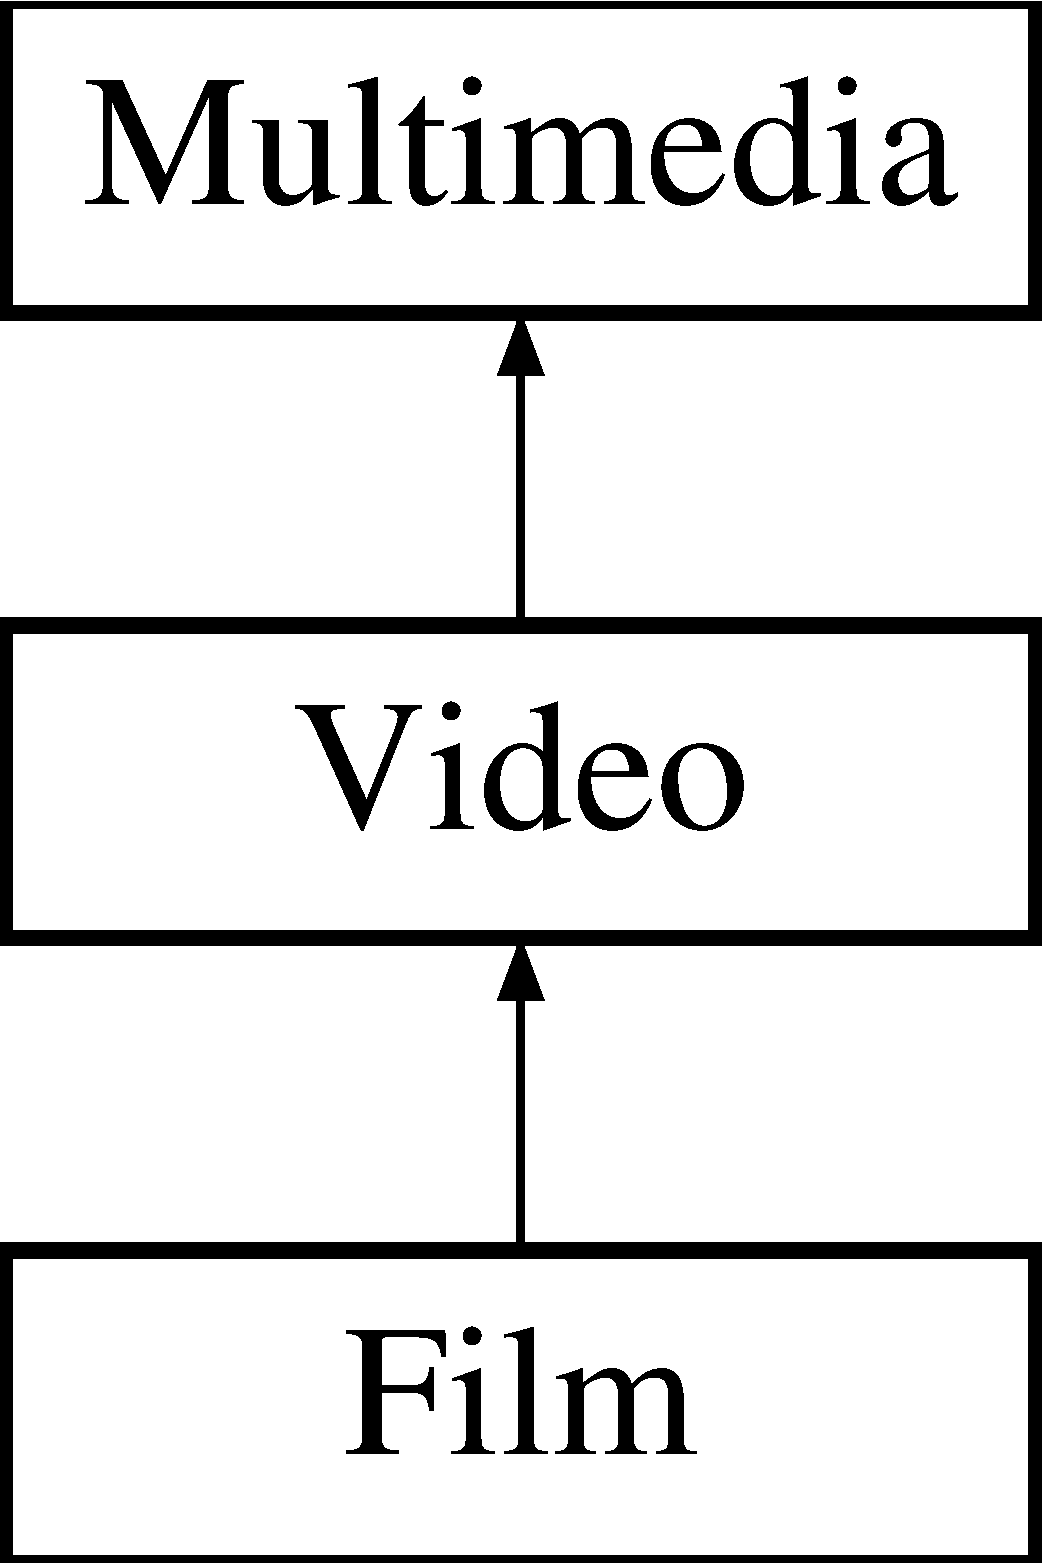
\includegraphics[height=3.000000cm]{class_video}
\end{center}
\end{figure}
\subsection*{Classes}
\begin{DoxyCompactItemize}
\item 
class \hyperlink{class_video_1_1_deleter_video}{Deleter\-Video}
\end{DoxyCompactItemize}
\subsection*{Public Member Functions}
\begin{DoxyCompactItemize}
\item 
virtual unsigned int \hyperlink{class_video_a3b3cfffbd171368fcfb70cd58bff60a8}{get\-Length} (void) const 
\begin{DoxyCompactList}\small\item\em Length getter. \end{DoxyCompactList}\item 
\hypertarget{class_video_a01da0b8e9ee9f91e515cf453f03b1bea}{virtual void {\bfseries set\-Length} (unsigned int new\-Length)}\label{class_video_a01da0b8e9ee9f91e515cf453f03b1bea}

\item 
virtual string \hyperlink{class_video_a9f6e63647c81fabd59452ad1d695d190}{print} (void) const 
\begin{DoxyCompactList}\small\item\em Print description. \end{DoxyCompactList}\item 
\hypertarget{class_video_a0bcf77c9b87b314385c95d92c3cba71e}{virtual void \hyperlink{class_video_a0bcf77c9b87b314385c95d92c3cba71e}{play} (void) const }\label{class_video_a0bcf77c9b87b314385c95d92c3cba71e}

\begin{DoxyCompactList}\small\item\em Display the multimedia file on screen. \end{DoxyCompactList}\item 
virtual void \hyperlink{class_video_a4bfb8bf83498fa30a6515065559ccbff}{write} (ostream \&stream) const 
\begin{DoxyCompactList}\small\item\em Serialize the multimedia object. \end{DoxyCompactList}\item 
virtual void \hyperlink{class_video_a6be318a4e05ddfdb52fbcc1cab5ab573}{read} (istream \&stream)
\begin{DoxyCompactList}\small\item\em Read from a serialized object. \end{DoxyCompactList}\end{DoxyCompactItemize}
\subsection*{Protected Member Functions}
\begin{DoxyCompactItemize}
\item 
\hypertarget{class_video_a77b13b3504ce1250d9d85988738d1ed3}{{\bfseries Video} (const \hyperlink{class_video}{Video} \&)}\label{class_video_a77b13b3504ce1250d9d85988738d1ed3}

\item 
\hyperlink{class_video_a0e0e31382d40c5f80e68d8441872eb56}{Video} (void)
\begin{DoxyCompactList}\small\item\em Default Constructor. \end{DoxyCompactList}\item 
\hyperlink{class_video_a11c9bacf664b637c4e3a214054df0ecf}{Video} (string name, unsigned long date, string pathname, unsigned int length)
\begin{DoxyCompactList}\small\item\em Constructor. \end{DoxyCompactList}\item 
virtual \hyperlink{class_video_a887b39f51487f64733e9541838118cf3}{$\sim$\-Video} (void)
\begin{DoxyCompactList}\small\item\em Destructor. \end{DoxyCompactList}\item 
virtual \hyperlink{class_video}{Video} $\ast$ \hyperlink{class_video_a450def61b99cd5c338b83cbfa136c25a}{clone} (void) const 
\begin{DoxyCompactList}\small\item\em Clone the video. \end{DoxyCompactList}\end{DoxyCompactItemize}
\subsection*{Friends}
\begin{DoxyCompactItemize}
\item 
\hypertarget{class_video_a29a97f20d6ded769adf9ecc47158e24f}{class {\bfseries Multimedia\-Manager}}\label{class_video_a29a97f20d6ded769adf9ecc47158e24f}

\item 
\hypertarget{class_video_ae6b99bde93d4652991dcd292ac9dcbd8}{class {\bfseries Deleter\-Video}}\label{class_video_ae6b99bde93d4652991dcd292ac9dcbd8}

\end{DoxyCompactItemize}


\subsection{Detailed Description}
This class represents a video file. 

\subsection{Constructor \& Destructor Documentation}
\hypertarget{class_video_a0e0e31382d40c5f80e68d8441872eb56}{\index{Video@{Video}!Video@{Video}}
\index{Video@{Video}!Video@{Video}}
\subsubsection[{Video}]{\setlength{\rightskip}{0pt plus 5cm}Video\-::\-Video (
\begin{DoxyParamCaption}
\item[{void}]{}
\end{DoxyParamCaption}
)\hspace{0.3cm}{\ttfamily [protected]}}}\label{class_video_a0e0e31382d40c5f80e68d8441872eb56}


Default Constructor. 

Defaut constructor of a video. \hypertarget{class_video_a11c9bacf664b637c4e3a214054df0ecf}{\index{Video@{Video}!Video@{Video}}
\index{Video@{Video}!Video@{Video}}
\subsubsection[{Video}]{\setlength{\rightskip}{0pt plus 5cm}Video\-::\-Video (
\begin{DoxyParamCaption}
\item[{string}]{name, }
\item[{unsigned long}]{date, }
\item[{string}]{pathname, }
\item[{unsigned int}]{length}
\end{DoxyParamCaption}
)\hspace{0.3cm}{\ttfamily [protected]}}}\label{class_video_a11c9bacf664b637c4e3a214054df0ecf}


Constructor. 

Constructor of a video.


\begin{DoxyParams}{Parameters}
{\em name} & \-: Name of the video. \\
\hline
{\em date} & \-: Date when the file is added. \\
\hline
{\em pathname} & \-: Path to the video. \\
\hline
{\em length} & \-: Length of the video in seconds. \\
\hline
\end{DoxyParams}
\hypertarget{class_video_a887b39f51487f64733e9541838118cf3}{\index{Video@{Video}!$\sim$\-Video@{$\sim$\-Video}}
\index{$\sim$\-Video@{$\sim$\-Video}!Video@{Video}}
\subsubsection[{$\sim$\-Video}]{\setlength{\rightskip}{0pt plus 5cm}Video\-::$\sim$\-Video (
\begin{DoxyParamCaption}
\item[{void}]{}
\end{DoxyParamCaption}
)\hspace{0.3cm}{\ttfamily [protected]}, {\ttfamily [virtual]}}}\label{class_video_a887b39f51487f64733e9541838118cf3}


Destructor. 

Default destructor of this class. 

\subsection{Member Function Documentation}
\hypertarget{class_video_a450def61b99cd5c338b83cbfa136c25a}{\index{Video@{Video}!clone@{clone}}
\index{clone@{clone}!Video@{Video}}
\subsubsection[{clone}]{\setlength{\rightskip}{0pt plus 5cm}{\bf Video} $\ast$ Video\-::clone (
\begin{DoxyParamCaption}
\item[{void}]{}
\end{DoxyParamCaption}
) const\hspace{0.3cm}{\ttfamily [protected]}, {\ttfamily [virtual]}}}\label{class_video_a450def61b99cd5c338b83cbfa136c25a}


Clone the video. 

\begin{DoxyReturn}{Returns}
Return a copy of the given video. 
\end{DoxyReturn}


Implements \hyperlink{class_multimedia_a2955c15860b8310ee684d391e7b3386f}{Multimedia}.



Reimplemented in \hyperlink{class_film_aa0b3eb1efeba4721d86c37ae5e671382}{Film}.

\hypertarget{class_video_a3b3cfffbd171368fcfb70cd58bff60a8}{\index{Video@{Video}!get\-Length@{get\-Length}}
\index{get\-Length@{get\-Length}!Video@{Video}}
\subsubsection[{get\-Length}]{\setlength{\rightskip}{0pt plus 5cm}unsigned int Video\-::get\-Length (
\begin{DoxyParamCaption}
\item[{void}]{}
\end{DoxyParamCaption}
) const\hspace{0.3cm}{\ttfamily [virtual]}}}\label{class_video_a3b3cfffbd171368fcfb70cd58bff60a8}


Length getter. 

Get the length of the video.

\begin{DoxyReturn}{Returns}
The length of the video. 
\end{DoxyReturn}
\hypertarget{class_video_a9f6e63647c81fabd59452ad1d695d190}{\index{Video@{Video}!print@{print}}
\index{print@{print}!Video@{Video}}
\subsubsection[{print}]{\setlength{\rightskip}{0pt plus 5cm}string Video\-::print (
\begin{DoxyParamCaption}
\item[{void}]{}
\end{DoxyParamCaption}
) const\hspace{0.3cm}{\ttfamily [virtual]}}}\label{class_video_a9f6e63647c81fabd59452ad1d695d190}


Print description. 

Print the description of the file to the standard output \begin{DoxyReturn}{Returns}
Return a string which contains the file description. 
\end{DoxyReturn}


Reimplemented from \hyperlink{class_multimedia_a4960a7ffd22e90f74291ebf86eccf820}{Multimedia}.

\hypertarget{class_video_a6be318a4e05ddfdb52fbcc1cab5ab573}{\index{Video@{Video}!read@{read}}
\index{read@{read}!Video@{Video}}
\subsubsection[{read}]{\setlength{\rightskip}{0pt plus 5cm}void Video\-::read (
\begin{DoxyParamCaption}
\item[{istream \&}]{stream}
\end{DoxyParamCaption}
)\hspace{0.3cm}{\ttfamily [virtual]}}}\label{class_video_a6be318a4e05ddfdb52fbcc1cab5ab573}


Read from a serialized object. 


\begin{DoxyParams}{Parameters}
{\em stream} & \-: the input stream where the object will be read. \\
\hline
\end{DoxyParams}


Implements \hyperlink{class_multimedia_ab686208e53fe8161bb86f7d37e01784c}{Multimedia}.



Reimplemented in \hyperlink{class_film_a053b2e4cd4b1e1f8dda7cfb1a45d301c}{Film}.

\hypertarget{class_video_a4bfb8bf83498fa30a6515065559ccbff}{\index{Video@{Video}!write@{write}}
\index{write@{write}!Video@{Video}}
\subsubsection[{write}]{\setlength{\rightskip}{0pt plus 5cm}void Video\-::write (
\begin{DoxyParamCaption}
\item[{ostream \&}]{stream}
\end{DoxyParamCaption}
) const\hspace{0.3cm}{\ttfamily [virtual]}}}\label{class_video_a4bfb8bf83498fa30a6515065559ccbff}


Serialize the multimedia object. 


\begin{DoxyParams}{Parameters}
{\em stream} & \-: the output stream where the object will be written. \\
\hline
\end{DoxyParams}


Implements \hyperlink{class_multimedia_aa3c800e85ac5256ee8d1399d2ba33329}{Multimedia}.



Reimplemented in \hyperlink{class_film_a8b38978dd0bf6ed844627d8e8b63efbe}{Film}.



The documentation for this class was generated from the following files\-:\begin{DoxyCompactItemize}
\item 
src/headers/video.\-h\item 
src/video.\-cpp\end{DoxyCompactItemize}

%--- End generated contents ---

% Index
\newpage
\phantomsection
\addcontentsline{toc}{chapter}{Index}
\printindex

\end{document}
